\documentclass[12pt]{article}
\usepackage[utf8]{inputenc}
\usepackage[spanish]{babel}
\usepackage{amsmath}
\usepackage{amssymb}
\usepackage{geometry}
\geometry{letterpaper, margin=2.5cm}
\usepackage{graphicx}
\usepackage{float}
\usepackage{fancyhdr}
\usepackage{enumitem}
\usepackage{multirow}
\usepackage{bigdelim}
\usepackage{subcaption, multicol}
\pagestyle{fancy}
\fancyhf{}
\setlength{\headheight}{40pt}
\lhead{\textbf{Grupo: 4CM4}}
\rhead{
        \footnotesize
        \begin{tabular}{r | l}
                Barrera Guerrero José Emanuel  & 2025630497 \\
                Romero Martínez Diego Enrique & 2025630526 \\
        \end{tabular}
}
\cfoot{\thepage}

\begin{document}

\begin{center}
        \Large \textbf{Teoría de la Computación} \\
        \large Periodo $2026/2$ \\
        \vspace{0.4cm}
        \Large \textbf{3ra Lista de problemas y ejercicios}
\end{center}

\section*{}Esta lista de problemas y ejercicios debe entregarse en formato PDF y se sugiere que sea realizada en computadora utilizando la herramienta JFLAP para diseñar y simular los autómatas y las expresiones regulares. En la parte superior de cada hoja debe aparecer la información general del alumno (nombre completo, boleta y grupo). Ademas, debe incluir las instrucciones y/o enunciados de cada ejercicio, no solo las respuestas. Finalmente, todas las respuestas de los ejercicios deben ir acompañadas del procedimiento y/o razonamiento.

NOTA: Los ejercicios que debe entregar en esta tarea son los que tienen un asterisco (*). El resto son opcionales.

\section*{Autómatas Finitos y Simplificación}
En los problemas 151-155, debe hallar el diagrama de transiciones del autómata definido en cada tabla y simplificarlo eliminando los estados que no son accesibles. A continuación, encontrará las tablas para cada uno de los problemas:

\begin{enumerate}
	\setcounter{enumi}{150}
	\item*
\end{enumerate}

		\begin{center}
		
		\begin{minipage}{0.30\textwidth}	
			\begin{center}
			\begin{tabular}{c|cc}
			Estado actual & 0 & 1 \\
			\hline
			$\rightarrow A$&$C$&$E$\\
			$B$ & $F$ & $E$\\
			$*C$&$A$&$G$\\
			$D$&$C$&$E$\\
			$*E$&$I$&$B$\\
			$*F$&$D$&$H$\\
			$G$&$F$&$I$\\
			$H$&$C$&$J$\\
			$I$&$J$&$E$\\
			$J$&$I$&$E$\\
			\end{tabular}
			\end{center}
			1. Asegurar que todos los estados sean accesibles, en caso que no lo sean quitarlos.
		\end{minipage}
		\hfill
		\begin{minipage}{0.60\textwidth}
		
			Esto es comprobado en la figura 1. Tambien podemos ver que cadenas son aceptadas y cuales no:
			\begin{figure}[H]
				\centering
				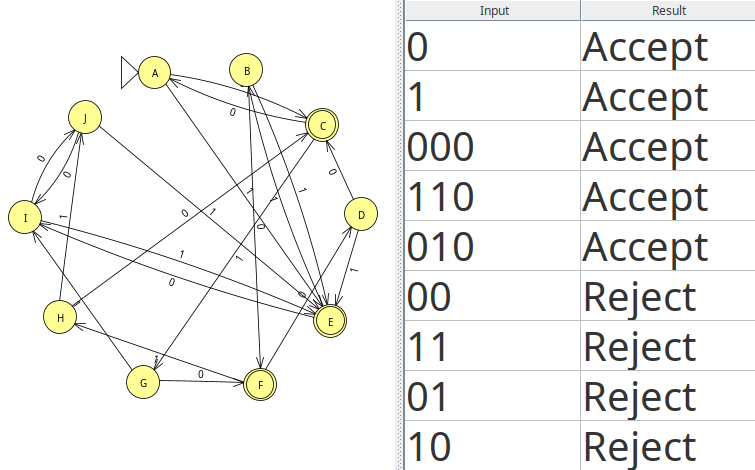
\includegraphics[width=0.8\textwidth]{imgs/ori151.png}
				\caption{Diagrama de transiciones y validacion en JFLAP No. 151.}
			\end{figure}
		\end{minipage}

		
		\vspace{0.5cm}
		\begin{minipage}{0.45\textwidth}
			2. Separar en scjtos 
			\begin{itemize}[noitemsep, label=-]
				\item Aceptación y no aceptación.
				\item siguientes iteraciones: Scjtos X2, X3, ...
			\end{itemize}
			$\rho_1 =\{x_0, x_1\}\\
			x_0=\{A, B, D, G, H, I, J\}\\
			x_1=\{C, E, F\}\\
			$

			3. Reescribir la tabla, separando en los conjuntos X0 y X1, (Xn según sea el caso) y reescribir las transiciones según el conjunto al que pertenezca la letra de transición en la tabla original.\\
			
			4. Hacer nuevos conjuntos de acuerdo con que su tabla de transiciones tenga la misma combinación de Scjtos.
		\end{minipage}
		\hfill
		\begin{minipage}{0.45\textwidth}
			\begin{center}
                        2da iteración\\
                        \vspace{0.5cm}
                        \begin{tabular}{c|cc l}
                        Estado actual & 0 & 1 &\\
                        \hline
                        $A$ & $x_1$ & $x_1$ & \rdelim\}{3}{*}[$x_2$]\\
                        $B$ & $x_1$ & $x_1$ &\\
                        $D$ & $x_1$ & $x_1$ &\\
                        $G$ & $x_1$ & $x_0$ & \rdelim\}{2}{*}[$x_3$]\\
                        $H$ & $x_1$ & $x_0$ &\\
                        $I$ & $x_0$ & $x_1$ & \rdelim\}{2}{*}[$x_4$]\\
                        $J$ & $x_0$ & $x_1$ &\\
                        \hline
                        $C$ & $x_0$ & $x_0$ & \rdelim\}{3}{*}[$x_5$]\\
                        $E$ & $x_0$ & $x_0$ &\\
                        $F$ & $x_0$ & $x_0$ &\\
                        \end{tabular}
                        \end{center}
                        $\rho_2=\{x_2,x_3,x_4,x_5\}\\
                        x_2=\{A, B, D\}\\
                        x_3=\{G, H\}\\
                        x_4=\{I, J\}\\
                        x_5=\{C, E, F\}\\
                        $
		\end{minipage}
		\vspace{0.5cm}

		\begin{minipage}{0.45\textwidth}
		5. Repetir los pasos 2, 3 y 4 hasta que ya no exista reducción posible (singuletes o que se empiezan a repetir grupos).
		\vspace{0.5cm}
		\begin{center}
			3ra iteración\\
                        \vspace{0.5cm}
                        \begin{tabular}{c|cc l}
                        Estado actual & 0 & 1 &\\
                        \hline
                        $A$ & $x_5$ & $x_5$ & \rdelim\}{3}{*}[$x_6$]\\
                        $B$ & $x_5$ & $x_5$ &\\
                        $D$ & $x_5$ & $x_5$ &\\
                        \hline
			$G$ & $x_5$ & $x_4$ & \rdelim\}{2}{*}[$x_7$]\\
                        $H$ & $x_5$ & $x_4$ &\\
                        \hline
			$I$ & $x_4$ & $x_5$ & \rdelim\}{2}{*}[$x_8$]\\
                        $J$ & $x_4$ & $x_5$ &\\
                        \hline
                        $C$ & $x_2$ & $x_3$ & $\rightarrow x_9$\\
                        $E$ & $x_4$ & $x_2$ & $\rightarrow x_{10}$\\
                        $F$ & $x_2$ & $x_3$ & $\rightarrow x_9$\\
                        \end{tabular}
                        \end{center}
                        $\rho_3=\{x_6,x_7,x_8,x_9,x_{10}\}\\
                        x_6=\{A, B, D\}\\
                        x_7=\{G, H\}\\
                        x_8=\{I, J\}\\
                        x_9=\{C, F\}\\
			x_{10}=\{E\}\\
                        $
		\end{minipage}	
			\hfill
		\begin{minipage}{0.45\textwidth}
		\begin{center}
                        4ta iteración\\
                        \vspace{0.5cm}
                        \begin{tabular}{c|cc l}
                        Estado actual & 0 & 1 &\\
                        \hline
                        $A$ & $x_9$ & $x_{10}$ & \rdelim\}{3}{*}[$x_{11}$]\\
                        $B$ & $x_9$ & $x_{10}$ &\\
                        $D$ & $x_9$ & $x_{10}$ &\\
                       	\hline
			$G$ & $x_9$ & $x_8$ & \rdelim\}{2}{*}[$x_{12}$]\\
                        $H$ & $x_9$ & $x_8$ &\\
                        \hline
			$I$ & $x_8$ & $x_{10}$ & \rdelim\}{2}{*}[$x_{13}$]\\
                        $J$ & $x_8$ & $x_{10}$ &\\
                        \hline
                        $C$ & $x_6$ & $x_7$ & \rdelim\}{2}{*}[$x_{14}$]\\
                        $F$ & $x_6$ & $x_7$ & \\
			\hline
			$E$ & $x_8$ & $x_6$ & $\rightarrow x_{15}$\\
                        \end{tabular}
                        \end{center}
                        $\rho_4=\{x_{11},x_{12},x_{13},x_{14},x_{15}\}\\
                        x_{11}=\{A, B, D\}\\
                        x_{12}=\{G, H\}\\
                        x_{13}=\{I, J\}\\  
                        x_{14}=\{C, F\}\\
                        x_{15}=\{E\}\\
                        $
		\end{minipage}

		\begin{minipage}{0.40\textwidth}
			\begin{center}
                        5ta iteración\\
                        \vspace{0.5cm}
                        \begin{tabular}{c|cc l}
                        Estado actual & 0 & 1 &\\
                        \hline
                        $A$ & $x_{14}$ & $x_{15}$ & \rdelim\}{3}{*}[$x_{16}$]\\
                        $B$ & $x_{14}$ & $x_{15}$ &\\
                        $D$ & $x_{14}$ & $x_{15}$ &\\
                        \hline
                        $G$ & $x_{14}$ & $x_{13}$ & \rdelim\}{2}{*}[$x_{17}$]\\
                        $H$ & $x_{14}$ & $x_{13}$ &\\
                        \hline
                        $I$ & $x_{13}$ & $x_{15}$ & \rdelim\}{2}{*}[$x_{18}$]\\
                        $J$ & $x_{13}$ & $x_{15}$ &\\
                        \hline
                        $C$ & $x_{11}$ & $x_{12}$ & \rdelim\}{2}{*}[$x_{19}$]\\
                        $F$ & $x_{11}$ & $x_{12}$ & \\
                        \hline
                        $E$ & $x_{13}$ & $x_{11}$ & $\rightarrow x_{20}$\\
                        \end{tabular}
                        \end{center}
                        $\rho_5=\{x_{16},x_{17},x_{18},x_{19},x_{20}\}\\
                        x_{16}=\{A, B, D\}\\
                        x_{17}=\{G, H\}\\
                        x_{18}=\{I, J\}\\
                        x_{19}=\{C, F\}\\
                        x_{20}=\{E\}\\
                        \rho_5=\rho_4
			$
		\end{minipage}
		\hfill
		\begin{minipage}{0.50\textwidth}
		Resultado final
		\begin{figure}[H]
		\centering
		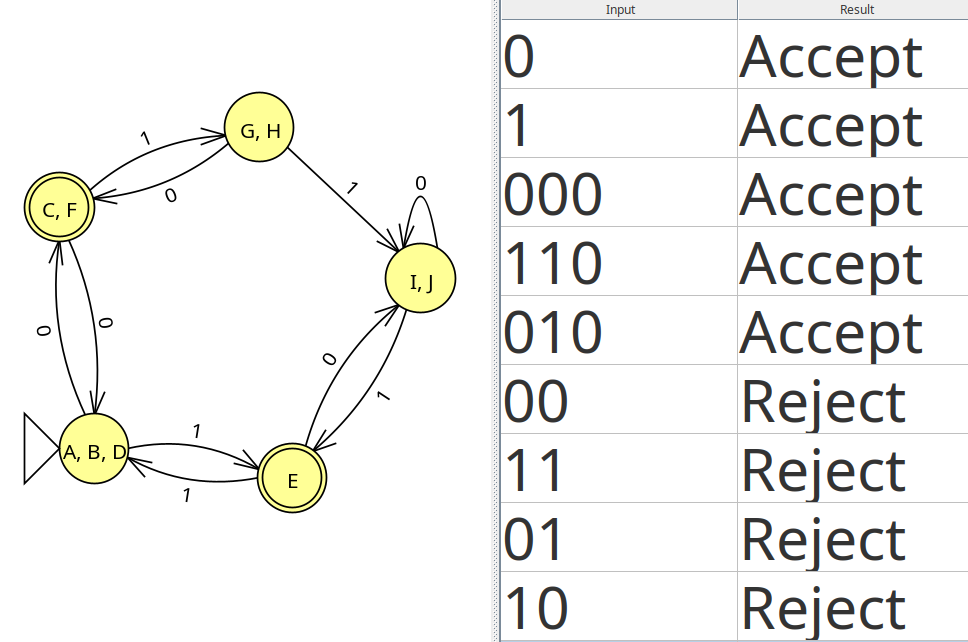
\includegraphics[width=0.9\textwidth]{imgs/final151.png}
		\caption{Diagrama de transiciones y validacion en JFLAP No. 151 simplificado.}		
		\end{figure}
		\end{minipage}	
		\end{center}
\begin{enumerate}		
\setcounter{enumi}{151}
\item*
\end{enumerate}		
		\begin{center}
		\begin{minipage}{0.45\textwidth}
			\begin{center}
			\begin{tabular}{c|ccc}
			Estado actual & 0 & 1 & 2\\
			\hline
			$\rightarrow A$ & $C$ & $E$ & $B$\\
			$B$ & $D$ & $E$ & $B$\\
			$C$ & $A$ & $D$ & $F$\\
			$*D$ & $F$ & $B$ & $C$\\
			$*E$ & $F$ & $B$ & $A$\\
			$*F$ & $D$ & $B$ & $C$\\
		\end{tabular}
		\end{center}
		En la siguiente figura se puede ver que todos los estados son accesibles:

		\end{minipage}
		\hfill
		\begin{minipage}{0.45\textwidth}	
		\begin{figure}[H]
		\centering
		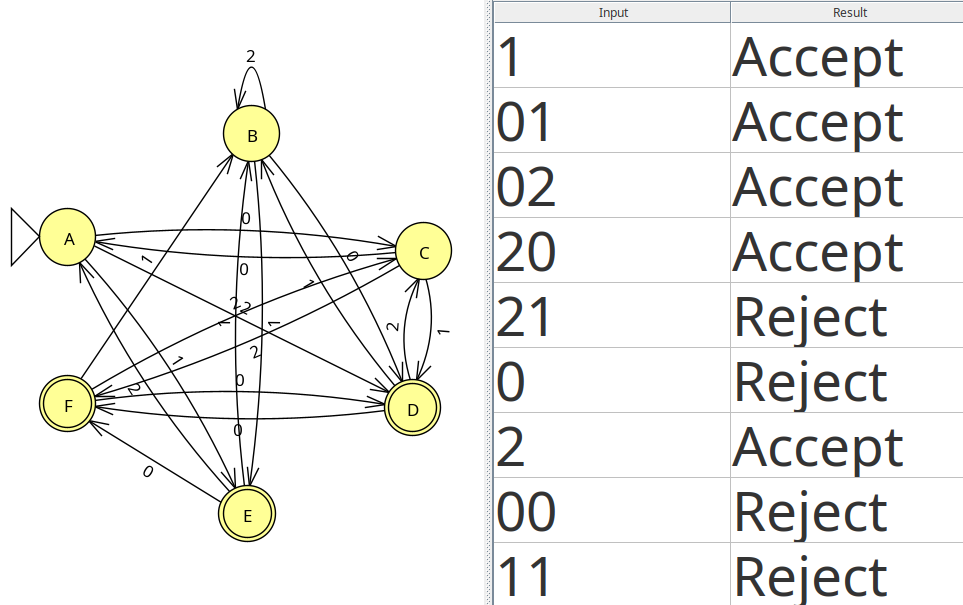
\includegraphics[width=0.8\textwidth]{imgs/ori152.png}
		\caption{Diagrama de transiciones y validacion en JFLAP No. 152.}
		\end{figure}
		\end{minipage}
		
		\vspace{0.5cm}
		\begin{minipage}{0.45\textwidth}
		$\rho_1=\{x_0, x_1\}$\\
		$x_0=\{A, B, C\}$\\
		$x_1=\{D, E, F\}$\\
		\end{minipage}
		\hfill
		\begin{minipage}{0.45\textwidth}
		\begin{center}
			2da iteración\\
			\vspace{0.5cm}
                        \begin{tabular}{c|ccc l}
                        Estado actual & 0 & 1 & 2\\
                        \hline
                        $A$ & $x_0$ & $x_1$ & $x_0$ & $\rightarrow x_2$\\
                        $B$ & $x_1$ & $x_1$ & $x_0$ & $\rightarrow x_3$\\
                        $C$ & $x_0$ & $x_1$ & $x_1$ & $\rightarrow x_4$\\
			\hline
                        $D$ & $x_1$ & $x_0$ & $x_0$ & \rdelim\}{3}{*}[$x_5$]\\
                        $E$ & $x_1$ & $x_0$ & $x_0$ &\\
                        $F$ & $x_1$ & $x_0$ & $x_0$ &\\
                \end{tabular}
                \end{center}
                \end{minipage}

		\begin{minipage}{0.45\textwidth}
		$\rho_2=\{x_2, x_3, x_4, x_5\}$\\
                $x_2=\{A\}$\\
		$x_3=\{B\}$\\
		$x_4=\{C\}$\\
                $x_5=\{D, E, F\}$\\

		\begin{center}
		3ra iteración\\
			\vspace{0.5cm}
                        \begin{tabular}{c|ccc l}   
                        Estado actual & 0 & 1 & 2\\
                        \hline
                        $A$ & $x_4$ & $x_5$ & $x_3$ & $\rightarrow x_6$\\
                        $B$ & $x_5$ & $x_5$ & $x_3$ & $\rightarrow x_7$\\
                        $C$ & $x_2$ & $x_5$ & $x_5$ & $\rightarrow x_8$\\
                        $D$ & $x_5$ & $x_3$ & $x_4$ & $\rightarrow x_9$\\
			\hline
                        $E$ & $x_5$ & $x_3$ & $x_2$ & \rdelim\}{2}{*}[$x_{10}$]\\
                        $F$ & $x_5$ & $x_3$ & $x_4$\\
                \end{tabular}
		\end{center}
		 $\rho_3=\{x_6, x_7, x_8, x_9, x_{10}\}$\\
                $x_6=\{A\}$\\
                $x_7=\{B\}$\\
                $x_8=\{C\}$\\
		$x_9=\{D\}$\\
                $x_{10}=\{E, F\}$\\

		\end{minipage}
		\hfill
		\begin{minipage}{0.45\textwidth}
			\begin{center} 
	                4ta iteración\\
                        \vspace{0.5cm}
                        \begin{tabular}{c|ccc l}
                        Estado actual & 0 & 1 & 2\\
                        \hline
                        $A$ & $x_8$ & $x_{10}$ & $x_7$ & $\rightarrow x_{11}$\\
                        $B$ & $x_9$ & $x_{10}$ & $x_7$ & $\rightarrow x_{12}$\\
                        $C$ & $x_6$ & $x_9$ & $x_{10}$ & $\rightarrow x_{13}$\\
                        $D$ & $x_{10}$ & $x_7$ & $x_8$ & $\rightarrow x_{14}$\\
                        $E$ & $x_{10}$ & $x_7$ & $x_6$ & $\rightarrow x_{15}$\\
                        $F$ & $x_9$ & $x_7$ & $x_8$ & $\rightarrow x_{16}$\\

                \end{tabular}
                \end{center} 
                 $\rho_4=\{x_{11}, x_{12}, x_{13}, x_{14}, x_{15}, x_{16}\}$\\
                $x_{11}=\{A\}$\\
                $x_{12}=\{B\}$\\
                $x_{13}=\{C\}$\\
                $x_{14}=\{D\}$\\
                $x_{15}=\{E\}$\\
		$x_{16}=\{F\}$\\

		Tras aplicar el algoritmo de minimización por particiones, se determinó que todos los estados son distinguibles entre sí. Por lo tanto, el autómata original ya se encuentra en su forma mínima y no es reducible; el diagrama de transiciones final es idéntico al inicial.
		\end{minipage}
                \end{center}
\begin{enumerate}		
\setcounter{enumi}{152}
    \item*
\end{enumerate}
    \begin{center}
        \begin{minipage}{0.30\textwidth}
            \begin{center}
            \begin{tabular}{c|cc}
            Estado actual & 0 & 1 \\
            \hline
            $\rightarrow A$&$B$&$C$\\
            $B$ & $D$ & $E$\\
            $C$ & $F$ & $G$\\
            $*D$&$D$&$E$\\
            $E$&$F$&$G$\\
            $*F$&$E$&$D$\\
            $*G$&$F$&$G$\\
            \end{tabular}
            \end{center}
        \end{minipage}
        \hfill
        \begin{minipage}{0.60\textwidth}
	En la siguiente figura se puede ver que todos los estados son accesibles:
            \begin{figure}[H]
                \centering
                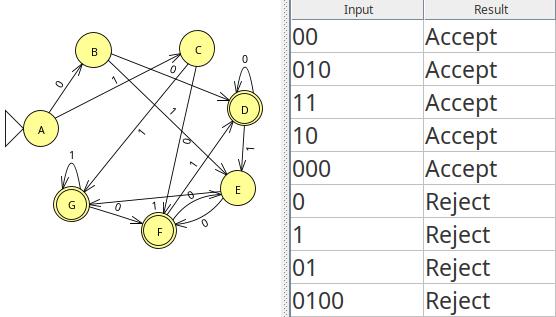
\includegraphics[width=0.8\textwidth]{imgs/ori153.png}
                \caption{Diagrama de transiciones y validacion en JFLAP No. 153.}
            \end{figure}
        \end{minipage}

        \vspace{0.5cm}
        \begin{minipage}{0.45\textwidth}
            $\rho_1 =\{x_0, x_1\}$\\
            $x_0=\{A, B, C, E\}$\\
            $x_1=\{D, F, G\}$\\
	\vspace{0.3cm}
	\begin{center}
            2da iteración\\
            \vspace{0.5cm}
            \begin{tabular}{c|cc l}
            Estado actual & 0 & 1 &\\
            \hline
            $A$ & $x_0$ & $x_0$ & $\rightarrow x_2$\\
            $B$ & $x_1$ & $x_0$ & $\rightarrow x_3$\\
	    \hline
            $C$ & $x_1$ & $x_1$ & \rdelim\}{2}{*}[$x_4$]\\
            $E$ & $x_1$ & $x_1$ &\\
            \hline
            $D$ & $x_1$ & $x_0$ & $\rightarrow x_5$\\
            $F$ & $x_0$ & $x_1$ & $\rightarrow x_6$\\
            $G$ & $x_1$ & $x_1$ & $\rightarrow x_7$\\
            \end{tabular}
            \end{center}
		 $\rho_2=\{x_2,x_3,x_4,x_5,x_6,x_7\}$\\
       		 $x_2=\{A\}$\\
        	 $x_3=\{B\}$\\
        	 $x_4=\{C, E\}$\\
        	 $x_5=\{D\}$\\
        	 $x_6=\{F\}$\\
	         $x_7=\{G\}$\\

        \end{minipage}
        \hfill
        \begin{minipage}{0.45\textwidth}
	    \begin{center}
            3ra iteración\\
            \vspace{0.5cm}
            \begin{tabular}{c|cc l}
            Estado actual & 0 & 1 &\\
            \hline
            $A$ & $x_3$ & $x_4$ & $\rightarrow x_8$\\
            $B$ & $x_5$ & $x_4$ & $\rightarrow x_9$\\
            $C$ & $x_6$ & $x_7$ & \rdelim\}{2}{*}[$x_{10}$]\\
            $E$ & $x_6$ & $x_7$ &\\
            $D$ & $x_5$ & $x_4$ & $\rightarrow x_{11}$\\
            $F$ & $x_4$ & $x_5$ & $\rightarrow x_{12}$\\
            $G$ & $x_6$ & $x_7$ & $\rightarrow x_{13}$\\
            \end{tabular}
            \end{center}
		$\rho_3=\{x_8,x_9,x_{10},x_{11},x_{12},x_{13}\}$\\
            $x_8=\{A\}$\\
            $x_9=\{B\}$\\
            $x_{10}=\{C, E\}$\\
            $x_{11}=\{D\}$\\
            $x_{12}=\{F\}$\\
            $x_{13}=\{G\}$\\
            $\rho_3 = \rho_2 \rightarrow$ Fin de la reducción.

        \end{minipage}

        \vspace{0.5cm}

        \begin{minipage}{0.50\textwidth}
            Resultado final
            \begin{figure}[H]
            \centering
            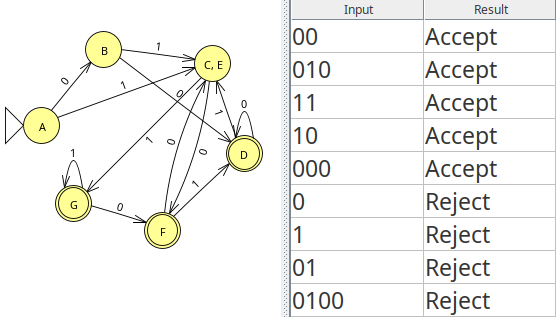
\includegraphics[width=0.9\textwidth]{imgs/final153.png}
            \caption{Diagrama de transiciones y validacion en JFLAP No. 153 simplificado.}
            \end{figure}
        \end{minipage}
    \end{center}
\newpage
\begin{enumerate}
    \setcounter{enumi}{153}
		\item *
		\begin{center}
		\begin{minipage}{0.45\textwidth}
			\begin{center}
			\begin{tabular}{c|ccc}
			Estado actual & 0 & 1\\
			\hline
			$\rightarrow A$ & $D$ & $K$\\
			$B$ & $H$ & $K$\\
			$C$ & $I$ & $E$\\
			$D$ & $C$ & $G$\\
			$*E$ & $K$ & $I$\\
			$F$ & $B$ & $E$\\
            $*G$ & $C$ & $I$\\
            $*H$ & $C$ & $B$\\
            $I$ & $G$ & $K$\\
            $*J$ & $F$ & $B$\\
            $K$ & $C$ & $F$\\
		      \end{tabular}
		      \end{center}
		De la tabla podemos concluir que el estado 'J' es el único estado inaccesible, por tanto lo quitamos de la tabla, resultando:
		\end{minipage}
        \hfill
        \begin{minipage}{0.45\textwidth}
		      \begin{center}
			\begin{tabular}{c|cc l}
			Estado actual & 0 & 1\\
			\hline
			$\rightarrow A$ & $D$ & $K$\\
			$B$ & $H$ & $K$\\
			$C$ & $I$ & $E$\\
			$D$ & $C$ & $G$\\
			$*E$ & $K$ & $I$\\
			$F$ & $B$ & $E$\\
            $*G$ & $C$ & $I$\\
            $*H$ & $C$ & $B$\\
            $I$ & $G$ & $K$\\
            $K$ & $C$ & $F$\\
		      \end{tabular}
		      \end{center}
	\end{minipage}
    \hfill
    \begin{minipage}{0.45\textwidth}	
		\begin{figure}[H]
		\centering
		
\includegraphics[width=1\textwidth]{imgs/ImgEma/ori154.png}
		\caption{Diagrama de transiciones y validación en JFLAP No. 154.}
		\end{figure}
		$\rho_1=\{x_0, x_1\}$\\
		$x_0=\{A,B,C,D,F,I,K\}$\\
		$x_1=\{E,G,H\}$\\
    \end{minipage}
    \hfill
    \begin{minipage}{0.45\textwidth}
		      \begin{center}
			2da iteración\\
			\vspace{0.5cm}
                \begin{tabular}{c|cc l}
    			Estado actual & 0 & 1\\
    			\hline
    			$A$ & $x_0$ & $x_0$ & $\rightarrow x_2$\\
    			$B$ & $x_1$ & $x_0$ & $\rightarrow x_3$\\
    			$C$ & $x_0$ & $x_1$ & \rdelim\}{3}{*}[$x_{4}$]\\
    			$D$ & $x_0$ & $x_1$\\
                $F$ & $x_0$ & $x_1$\\
                $I$ & $x_1$ & $x_0$ & $\rightarrow x_3$\\
                $K$ & $x_0$ & $x_0$ & $\rightarrow x_2$\\
                \hline
    			$E$ & $x_0$ & $x_0$ & \rdelim\}{3}{*}[$x_{5}$]\\
                $G$ & $x_0$ & $x_0$\\
                $H$ & $x_0$ & $x_0$\\
    		      \end{tabular}
            \end{center}
		$\rho_2=\{x_2, x_3, x_4\}$\\
        $x_2=\{A,K\}$\\
		$x_3=\{B,I\}$\\
		$x_4=\{C,D,F\}$\\
        $x_5=\{E,G,H\}$\\
    \end{minipage}
    \hfill
    \begin{minipage}{0.45\textwidth}
		\begin{center}
        \vspace{0.5cm}
		3ra iteración\\
            \begin{tabular}{c|cc l}
    			Estado actual & 0 & 1\\
    			\hline
    			$A$ & $x_4$ & $x_2$ & $\rightarrow x_6$\\
    			$K$ & $x_4$ & $x_4$ & $\rightarrow x_7$\\
                \hline
    			$B$ & $x_5$ & $x_2$ & \rdelim\}{2}{*}[$x_{8}$]\\
    			$I$ & $x_5$ & $x_2$ &\\
                \hline
                $C$ & $x_3$ & $x_5$ & $\rightarrow x_9$\\
                $D$ & $x_4$ & $x_5$ & $\rightarrow x_{10}$\\
                $F$ & $x_3$ & $x_5$ & $\rightarrow x_9$\\
                \hline
    			$E$ & $x_2$ & $x_3$ & $\rightarrow x_{11}$\\
                $G$ & $x_4$ & $x_3$ & \rdelim\}{2}{*}[$x_{12}$]\\
                $H$ & $x_4$ & $x_3$\\
    		\end{tabular}
		\end{center}
	$\rho_3=\{x_6, x_7, x_8, x_9, x_{10}, x_{11}, x_{12}\}$\\
    $x_6=\{A\}$\\
    $x_7=\{K\}$\\
    $x_8=\{B,I\}$\\
    $x_9=\{C,F\}$\\
    $x_{10}=\{D\}$\\
    $x_{11}=\{E\}$\\
    $x_{12}=\{G,H\}$\\
    
		\begin{center} 
	    4ta iteración\\
        \vspace{0.5cm}
        \begin{tabular}{c|cc l}
    			Estado actual & 0 & 1\\
    			\hline
    			$A$ & $x_{10}$ & $x_7$ & $\rightarrow x_{13}$\\
                \hline
    			$K$ & $x_9$ & $x_9$ & $\rightarrow x_{14}$\\
                \hline
    			$B$ & $x_{12}$ & $x_7$ & \rdelim\}{2}{*}[$x_{15}$]\\
    			$I$ & $x_{12}$ & $x_7$\\
                \hline
                $C$ & $x_8$ & $x_{11}$ & \rdelim\}{2}{*}[$x_{16}$]\\
                $F$ & $x_8$ & $x_{11}$\\
                \hline
                $D$ & $x_9$ & $x_{12}$ & $\rightarrow x_{17}$\\
                \hline
    			$E$ & $x_7$ & $x_8$ & $\rightarrow x_{18}$\\
                \hline
                $G$ & $x_9$ & $x_8$ & \rdelim\}{2}{*}[$x_{19}$]\\
                $H$ & $x_9$ & $x_8$\\
    		\end{tabular}
        \end{center} 
    $\rho_4=\{x_{13}, x_{14}, x_{15}, x_{16}, x_{17}, x_{18}, x_{19}\}$\\
    $x_{13}=\{A\}$\\
    $x_{14}=\{K\}$\\
    $x_{15}=\{B,I\}$\\
    $x_{16}=\{C,F\}$\\
    $x_{17}=\{D\}$\\
    $x_{18}=\{E\}$\\
    $x_{19}=\{G,H\}$
    \end{minipage}
    \hfill
    \begin{minipage}{0.45\textwidth}
    \begin{center}
        \textbf{5ta iteración} \\[0.5cm]
        \begin{tabular}{c|cc l}
            Estado actual & 0 & 1 & \\
            \hline
            $A$ & $x_{17}$ & $x_{14}$ & $\rightarrow x_{20}$\\
            \hline
            $K$ & $x_{16}$ & $x_{16}$ & $\rightarrow x_{21}$\\
            \hline
            $B$ & $x_{19}$ & $x_{14}$ & \rdelim\}{2}{1.5cm}[$x_{22}$] \\
            $I$ & $x_{19}$ & $x_{14}$ & \\
            \hline
            $C$ & $x_{15}$ & $x_{18}$ & \rdelim\}{2}{1.5cm}[$x_{23}$] \\
            $F$ & $x_{15}$ & $x_{18}$ & \\
            \hline
            $D$ & $x_{15}$ & $x_{19}$ & $\rightarrow x_{24}$\\
            \hline
            $E$ & $x_{14}$ & $x_{15}$ & $\rightarrow x_{25}$\\
            \hline
            $G$ & $x_{16}$ & $x_{15}$ & \rdelim\}{2}{1.5cm}[$x_{26}$] \\
            $H$ & $x_{16}$ & $x_{15}$ & \\
        \end{tabular}
    \end{center}
    $\rho_5=\{x_{20}, x_{21}, x_{22}, x_{23}, x_{24}, x_{25}, x_{26}\}$\\
    $x_{20}=\{A\}$\\
    $x_{21}=\{K\}$\\
    $x_{22}=\{B,I\}$\\
    $x_{23}=\{C,F\}$\\
    $x_{24}=\{D\}$\\
    $x_{25}=\{E\}$\\
    $x_{26}=\{G,H\}$\\    
\end{minipage}
\hfill
\begin{minipage}{0.45\textwidth}
    \begin{figure}[H]
		\centering
		
\includegraphics[width=1.2\textwidth]{imgs/ImgEma/final154.png}
		\caption{Diagrama de transiciones simplificado y estados de validación.}
    \end{figure}
\end{minipage}
\end{center}
\end{enumerate}

\begin{enumerate}
\setcounter{enumi}{154}
    \item*
    \begin{center}
        \begin{minipage}{0.30\textwidth}
            \begin{center}
            \begin{tabular}{c|cc}
            Estado actual & 0 & 1 \\
            \hline
            $\rightarrow A$&$B$&$C$\\
            $B$ & $D$ & $E$\\
            $C$ & $K$ & $G$\\
            $D$ & $H$ & $E$\\
            $E$ & $F$ & $D$\\
            $*F$ & $J$ & $G$\\
            $G$ & $E$ & $G$\\
            $H$ & $B$ & $K$\\
            $I$ & $C$ & $A$\\
            $J$ & $D$ & $G$\\
            $K$ & $F$ & $D$\\
            $L$ & $C$ & $J$\\
            \end{tabular}
            \end{center}
        \end{minipage}
        \hfill
        \begin{minipage}{0.60\textwidth}
        Los estados $I$ y $L$ son inaccesibles desde el estado inicial, por lo que se eliminan para la minimización.
            \begin{figure}[H]
                \centering
                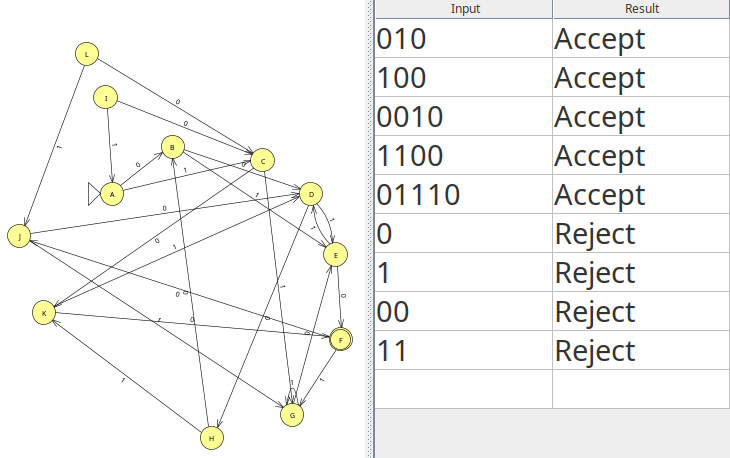
\includegraphics[width=0.8\textwidth]{imgs/ori155.png}
                \caption{Diagrama de transiciones y validación en JFLAP No. 155.}
            \end{figure}
        \end{minipage}

        \vspace{0.5cm}
	\hfill
	\vspace{0.5cm}
        \begin{minipage}{0.45\textwidth}
            $\rho_1 =\{x_0, x_1\}$\\
            $x_0=\{A, B, C, D, E, G, H, J, K\}$\\
            $x_1=\{F\}$\\
        \vspace{0.3cm}
        \begin{center}
            2da iteración\\
            \vspace{0.5cm}
            \begin{tabular}{c|cc l}
            Estado actual & 0 & 1 &\\
            \hline
            $A$ & $x_0$ & $x_0$ & \rdelim\}{7}{*}[$x_2$]\\
            $B$ & $x_0$ & $x_0$ &\\
            $C$ & $x_0$ & $x_0$ &\\
            $D$ & $x_0$ & $x_0$ &\\
            $G$ & $x_0$ & $x_0$ &\\
            $H$ & $x_0$ & $x_0$ &\\
            $J$ & $x_0$ & $x_0$ &\\
	    \hline
            $E$ & $x_1$ & $x_0$ & \rdelim\}{2}{*}[$x_3$]\\
            $K$ & $x_1$ & $x_0$ &\\
	    \hline
            $F$ & $x_0$ & $x_0$ & $\rightarrow x_4$\\

            \end{tabular}
            \end{center}
		$\rho_2=\{x_2,x_3,x_4\}$\\
		$x_2=\{A, B, C, D, G, H, J\}$\\
		$x_3=\{E, K\}$\\
                $x_2=\{F\}$\\
	\end{minipage}
	\hfill
	\begin{minipage}{0.45\textwidth}
        \vspace{0.3cm}
        \begin{center}
            3ra iteración\\
            \vspace{0.5cm}
            \begin{tabular}{c|cc l}
            Estado actual & 0 & 1 &\\
            \hline
            $A$ & $x_2$ & $x_2$ & \rdelim\}{2}{*}[$x_5$]\\
            $J$ & $x_2$ & $x_2$ &\\
            \hline
            $B$ & $x_2$ & $x_3$ & \rdelim\}{3}{*}[$x_6$]\\
            $D$ & $x_2$ & $x_3$ &\\
            $H$ & $x_2$ & $x_3$ &\\
            \hline
            $C$ & $x_3$ & $x_2$ & \rdelim\}{2}{*}[$x_7$]\\
            $G$ & $x_3$ & $x_2$ &\\
	    \hline
            $E$ & $x_4$ & $x_2$ & \rdelim\}{2}{*}[$x_8$]\\
            $K$ & $x_4$ & $x_2$ &\\
	    \hline
            $F$ & $x_2$ & $x_2$ & $\rightarrow x_9$\\

            \end{tabular}
            \end{center}
                $\rho_3=\{x_5,x_6,x_7,x_8,x_9\}$\\
            $x_5=\{A, J\}$\\
            $x_6=\{B, D, H\}$\\
            $x_7=\{C, G\}$\\
	    $x_9=\{F\}$\\
            $x_8=\{E, K\}$\\

        \end{minipage}
        \hfill
        \begin{minipage}{0.45\textwidth}
            \begin{center}
            4ta iteración\\
            \vspace{0.5cm}
            \begin{tabular}{c|cc l}
            Estado actual & 0 & 1 &\\
		\hline
            $A$ & $x_6$ & $x_7$ & \rdelim\}{2}{*}[$x_{10}$]\\
            $J$ & $x_6$ & $x_7$ &\\
            \hline
            $B$ & $x_6$ & $x_8$ & \rdelim\}{3}{*}[$x_{11}$]\\
            $D$ & $x_6$ & $x_8$ &\\
            $H$ & $x_6$ & $x_8$ &\\
            \hline
            $C$ & $x_8$ & $x_7$ & \rdelim\}{2}{*}[$x_{12}$]\\
            $G$ & $x_8$ & $x_7$ &\\
            \hline
            $E$ & $x_9$ & $x_6$ & \rdelim\}{2}{*}[$x_{13}$]\\
            $K$ & $x_9$ & $x_6$ &\\
            \hline
            $F$ & $x_5$ & $x_7$ & $\rightarrow x_{14}$\\
            \end{tabular}
            \end{center}
                $\rho_4=\{x_{10},x_{11},x_{12},x_{13},x_{14}\}$\\
                $x_{10}=\{A, J\}$\\
                $x_{11}=\{B, D, H\}$\\
                $x_{12}=\{C, G\}$\\
    	          $x_{13}=\{E, K\}$\\
        	    $x_{14}=\{F\}$\\

            $\rho_4 = \rho_3 \rightarrow$ Fin de la reducción.

        \end{minipage}
	\hfill
        \begin{minipage}{0.45\textwidth}
            Resultado final
            \begin{figure}[H]
            \centering
            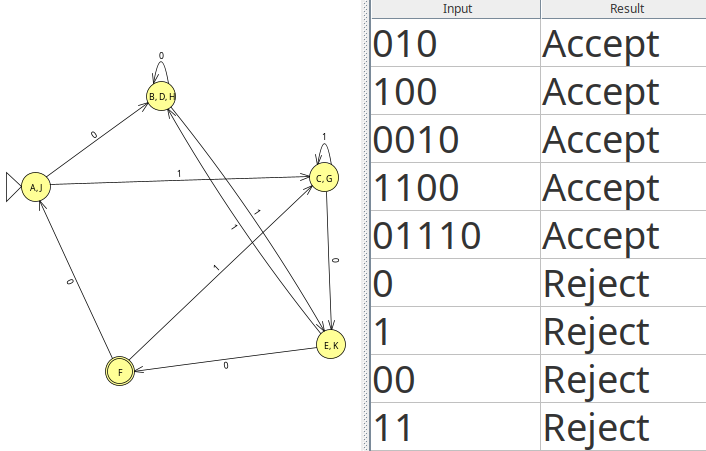
\includegraphics[width=0.9\textwidth]{imgs/final155.png}
            \caption{Diagrama de transiciones y validación en JFLAP No. 155 simplificado.}
            \end{figure}
        \end{minipage}
    \end{center}
\end{enumerate}
\vspace{0.3cm}
En los problemas 156-157, debe hallar la tabla de transiciones del autómata que se muestra y simplificarlo encontrando una partición, eliminando los estados que no son accesibles.
\begin{enumerate}
\setcounter{enumi}{155}
    \item*
    \begin{center}
        \begin{minipage}{0.45\textwidth}
            \begin{figure}[H]
    		\centering
    		
\includegraphics[width=1.2\textwidth]{imgs/ImgEma/ori156.png}
    		\caption{Diagrama de transiciones y estados de validación 156.}
            \end{figure}
        \end{minipage}
        \hfill
        \begin{minipage}{0.45\textwidth}
            \begin{center}
			\begin{tabular}{c|cc}
			Estado actual & 0 & 1\\
			\hline
			$\rightarrow A$ & $B$ & $C$\\
			$B$ & $C$ & $E$\\
			$C$ & $D$ & $C$\\
			$D$ & $C$ & $E$\\
			$*E$ & $B$ & $E$\\
		      \end{tabular}
		      \end{center}
        \end{minipage}
    \end{center}
\end{enumerate}
\vspace{0.5cm}
Tanto del autómata, como de la tabla de transiciones notamos que no existen estados inaccesibles, por ende empezamos separando los estados de transición y aceptación.
\begin{center}
    \begin{minipage}{0.45\textwidth}
        \begin{center}
		\begin{tabular}{c|cc l}
		Estado actual & 0 & 1\\
		\hline
        $\rightarrow A$ & $B$ & $C$ & \rdelim\}{4}{1.5cm}[$x_{0}$]\\
		$B$ & $C$ & $E$\\
		$C$ & $D$ & $C$\\
        $D$ & $C$ & $E$\\
		$*E$ & $B$ & $E$ & $\rightarrow x_{1}$\\
        \end{tabular}
        \end{center}
    \end{minipage}
    \hfill
    \begin{minipage}{0.45\textwidth}
        1ra iteración.\\
        $\rho_0=\{x_{0}, x_{1}\}$\\
        $x_{0}=\{A,B,C,D\}$\\
        $x_{1}=\{E\}$\\
    \end{minipage}
    \hfill\vspace{0.5cm}
    \begin{minipage}{0.45\textwidth}
        \begin{center}
		\begin{tabular}{c|cc l}
		Estado actual & 0 & 1\\
		\hline
        $A$ & $x_0$ & $x_0$ & $\rightarrow x_{2}$\\
		$B$ & $x_0$ & $x_1$ & $\rightarrow x_{3}$\\
		$C$ & $x_0$ & $x_0$ & $\rightarrow x_{2}$\\
        $D$ & $x_0$ & $x_1$ & $\rightarrow x_{3}$\\
        \hline
		$E$ & $x_0$ & $x_1$ & $\rightarrow x_{4}$\\
        \end{tabular}
        \end{center}
    \end{minipage}
    \hfill\vspace{0.5cm}
    \begin{minipage}{0.45\textwidth}
        2da iteración.\\
        $\rho_1=\{x_{2}, x_{3},x_4\}$\\
        $x_{2}=\{A,C\}$\\
        $x_{3}=\{B.D\}$\\
        $x_{4}=\{E\}$\\
    \end{minipage}
    \hfill
    \begin{minipage}{0.45\textwidth}
        \begin{center}
		\begin{tabular}{c|cc l}
		Estado actual & 0 & 1\\
		\hline
        $A$ & $x_3$ & $x_2$ & \rdelim\}{2}{1.5cm}[$x_{5}$]\\
		$C$ & $x_3$ & $x_2$\\
        \hline
		$B$ & $x_2$ & $x_4$ & \rdelim\}{2}{1.5cm}[$x_{6}$]\\
        $D$ & $x_2$ & $x_4$\\
        \hline
		$E$ & $x_3$ & $x_4$ & $\rightarrow x_{7}$\\
        \end{tabular}
        \end{center}
    \end{minipage}
    \hfill\vspace{0.5cm}
    \begin{minipage}{0.45\textwidth}
        3ra iteración.\\
        $\rho_2=\{x_{5}, x_{6},x_7\}$\\
        $x_{5}=\{A,C\}$\\
        $x_{6}=\{B.D\}$\\
        $x_{7}=\{E\}$\\
    \end{minipage}
    \begin{figure}[H]
    	\centering
    	
\includegraphics[width=1\textwidth]{imgs/ImgEma/final156.png}
    	\caption{Diagrama simplificado y de transiciones con estados de validación.}
    \end{figure}
\end{center}
\clearpage
\vspace{0.5cm}
\begin{enumerate}
\setcounter{enumi}{156}
    \item*
\end{enumerate}


\vspace{0.3cm}
\begin{center}
\begin{minipage}{0.35\textwidth}
	
\begin{figure}[H]
            \centering
            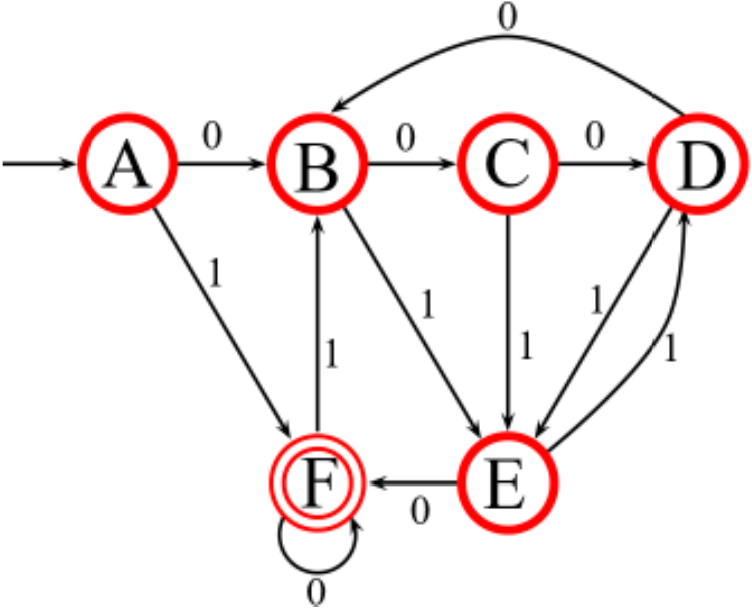
\includegraphics[width=0.9\textwidth]{imgs/157.png}
            \end{figure}
		\begin{center}
        \begin{tabular}{c|cc}
            Estado actual & 0 & 1 \\
                \hline
                $\rightarrow A$ & $B$ & $F$ \\
                $B$ & $C$ & $E$\\
                $C$ & $D$ & $E$\\
                $D$ & $B$ & $E$\\
                $E$ & $F$ & $D$\\
                \hline
                $*F$ & $F$ & $B$\\
            \end{tabular}
        \end{center}
\end{minipage}
\hfill
\begin{minipage}{0.55\textwidth}
	$\rho_1 =\{x_0, x_1\}\\
	x_0=\{A, B, C, D, E\}\\
	x_1=\{F\}\\
	$
		\begin{figure}[H]
		\centering
		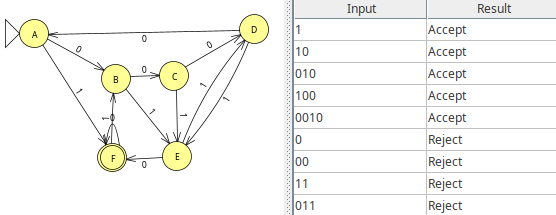
\includegraphics[width=0.9\textwidth]{imgs/ori157.png}
		\caption{Diagrama de transiciones y validacion en JFLAP No. 157.}
		\end{figure}
	\end{minipage}
	\begin{minipage}{0.45\textwidth}
		\begin{center}
		2da iteración\\
		\vspace{0.5cm}
		\begin{tabular}{c|cc l}
		Estado actual & 0 & 1 &\\
		\hline
		$A$ & $x_0$ & $x_1$ & $\rightarrow x_2$\\
		\hline
		$B$ & $x_0$ & $x_0$ & \rdelim\}{3}{*}[$x_3$]\\
		$C$ & $x_0$ & $x_0$ &\\
		$D$ & $x_0$ & $x_0$ &\\
		\hline
		$E$ & $x_1$ & $x_0$ & \rdelim\}{2}{*}[$x_4$]\\
		$F$ & $x_1$ & $x_0$ & \\
		\end{tabular}
		\end{center}
		$\rho_2=\{x_2, x_3, x_4\}\\
		x_2=\{A\}\\
		x_3=\{B, C, D\}\\
		x_4=\{E, F\}\\
		$
		\end{minipage}
		\hfill
		\begin{minipage}{0.45\textwidth}
		\begin{center}
		3ra iteración\\
		\vspace{0.5cm}
		\begin{tabular}{c|cc l}
		Estado actual & 0 & 1 &\\
		\hline
		$A$ & $x_3$ & $x_5$ & $\rightarrow x_5$\\
		\hline
		$B$ & $x_3$ & $x_4$ & \rdelim\}{3}{*}[$x_6$]\\
		$C$ & $x_3$ & $x_4$ &\\
		$D$ & $x_3$ & $x_4$ &\\
		\hline
		$E$ & $x_5$ & $x_3$ & \rdelim\}{2}{*}[$x_7$]\\
		$F$ & $x_5$ & $x_3$ & \\
		\end{tabular}
		\end{center}
		$\rho_3=\{x_5, x_6, x_7\}\\
		x_5=\{A\}\\
		x_6=\{B, C, D\}\\
		x_7=\{E, F\}\\
		\rho_3=\rho_2
		$
		\end{minipage}
		\begin{minipage}{0.45\textwidth}
		\vspace{0.5cm}
		Resultado final:
		\begin{figure}[H]
        	\centering
        	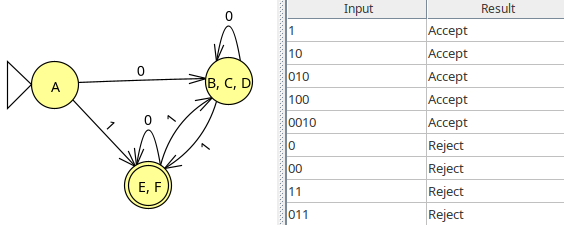
\includegraphics[width=0.9\textwidth]{imgs/final157.png}
        	\caption{Diagrama de transiciones y validacion simplificado.}
	\end{figure}
	\end{minipage}
\end{center}
\section*{Autómatas Finitos No Deterministas}
En los problemas 158-161, debe describir lo que hacen los autómatas finitos no deterministas definidos en cada tabla, donde el alfabeto es $\Sigma = \{0, 1\}$.

\begin{enumerate}
\setcounter{enumi}{157}
    \item*
    \begin{center}
        \begin{minipage}{0.45\textwidth}
            \begin{figure}[H]
    		\centering
    		
\includegraphics[width=1.2\textwidth]{imgs/ImgEma/Doc158.png}
    		\caption{Autómata 158.}
            \end{figure}
        \end{minipage}
        \hfill
        \begin{minipage}{0.45\textwidth}
            \begin{center}
			\begin{tabular}{c|cc}
			Estado actual & 0 & 1\\
			\hline
			$\rightarrow q1$ & $q2$ & $\emptyset$\\
			$q2$ & $\emptyset$ & $q3$\\
			$*q3$ & $\emptyset$ & $\emptyset$\\
		      \end{tabular}
		      \end{center}
        \end{minipage}
    \end{center}
\end{enumerate}
\centering El autómata solo acepta las cadenas $01$, específicamente esto es $L=\{01\}$, aquellas cadenas que contengan otros caracteres del alfabeto son rechazadas en automático.

\begin{enumerate}
\setcounter{enumi}{158}
\item*
\end{enumerate}
\begin{center}
\begin{minipage}{0.35\textwidth}
\begin{figure}[H]
                \centering
                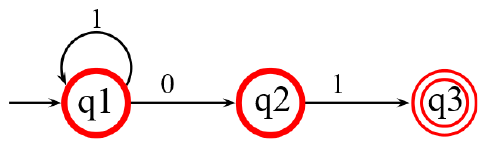
\includegraphics[width=0.9\textwidth]{imgs/159.png}
        \end{figure}
\begin{center}
\textbf{Tabla de transiciones} \\
            \vspace{0.3cm}
            \begin{tabular}{c|cc}
                Estado actual & 0 & 1 \\
                \hline
                $\rightarrow q_1$ & $\{q_2\}$ & $\{q_1\}$ \\
                $q_2$ & $\emptyset$ & $\{q_3\}$ \\
                $*q_3$ & $\emptyset$ & $\emptyset$ \\
            \end{tabular}
        \end{center}

\end{minipage}
\hfill
\begin{minipage}{0.55\textwidth}
\textbf{Descripción formal:}\\
        El lenguaje aceptado por este AFND está definido por la expresión regular $1^*01$. \\

\vspace{0.3cm}
\textbf{Descripción textual:}\\
        El autómata acepta todas las cadenas que inician con una cantidad indefinida de unos (incluyendo cero unos) y que finalizan estrictamente con la secuencia \textbf{01}. Al carecer de transiciones de salida en $q_3$, cualquier símbolo adicional posterior al 01 provocará el rechazo de la cadena.
\end{minipage}
\end{center}

\begin{enumerate}
\setcounter{enumi}{159}
    \item*
    \begin{center}
        \begin{minipage}{0.45\textwidth}
            \begin{figure}[H]
    		\centering
    		
\includegraphics[width=1.2\textwidth]{imgs/ImgEma/Doc160.png}
    		\caption{Autómata 160.}
            \end{figure}
        \end{minipage}
        \hfill
        \begin{minipage}{0.45\textwidth}
            \begin{center}
			\begin{tabular}{c|cc}
			Estado actual & 0 & 1\\
			\hline
			$\rightarrow q1$ & $q2$ & $\emptyset$\\
			$q2$ & $\emptyset$ & $q3$\\
			$*q3$ & $q3$ & $q3$\\
		      \end{tabular}
		      \end{center}
        \end{minipage}
    \end{center}
\end{enumerate}
\centering Este autómata solo acepta cadenas que comienzan unicamente con "01", esto es $L=\{01(0+1)^*$

\newpage
\begin{enumerate}
\setcounter{enumi}{160}
\item*
\end{enumerate}
\begin{center}
	\begin{minipage}{0.35\textwidth}
		\begin{figure}[H]
			\centering
			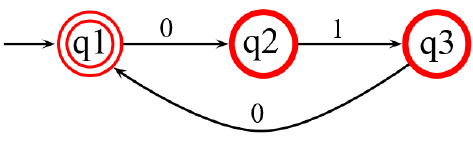
\includegraphics[width=0.9\textwidth]{imgs/161.png}
		\end{figure}

		\begin{center}
            \textbf{Tabla de transiciones} \\
            \vspace{0.3cm}
            \begin{tabular}{c|cc}
                Estado actual & 0 & 1 \\
                \hline
                $\rightarrow *q_1$ & $\{q_2\}$ & $\emptyset$ \\
                $q_2$ & $\emptyset$ & $\{q_3\}$ \\
                $q_3$ & $\{q_1\}$ & $\emptyset$ \\
            \end{tabular}
        \end{center}
	\end{minipage}
	\hfill
	\begin{minipage}{0.55\textwidth}
		\textbf{Descripción formal:}\\
        El lenguaje aceptado por este AFND está definido por la expresión regular $(010)^*$. \\

        \vspace{0.3cm}
        \textbf{Descripción textual:}\\
        El autómata acepta la cadena vacía ($\epsilon$) y cualquier cadena que esté formada exclusivamente por repeticiones sucesivas de la secuencia \textbf{010}. Cualquier alteración en este patrón provocará el rechazo inmediato de la cadena.
	\end{minipage}
	\end{center}

	\vspace{1.5cm}
	Los ejercicios 162-188 consisten en encontrar un autómata finito no determinista que haga lo que se pide en cada uno de los problemas 94-123 de la tarea 2, cuando sea posible, busque que el diagrama del AFN sea más simple que el del AFD. Como en la tarea 2, los problemas con * son obligatorios y el resto son optativos.

\begin{enumerate}
\setcounter{enumi}{161}
    \item Las palabras de $\Sigma_1$ que comienzan con 1 y terminan con 2.
    \begin{center}
        \begin{minipage}{0.45\textwidth}
            \begin{figure}[H]
    		\centering
    		
\includegraphics[width=1.2\textwidth]{imgs/ImgEma/AFN2L94.png}
            \end{figure}
        \end{minipage}
        \hfill
        \begin{minipage}{0.45\textwidth}
            \begin{center}
			\begin{tabular}{c|ccc}
			Estado actual & 0 & 1 & 2\\
			\hline
			$\rightarrow q0$ & $\emptyset$ & $q1$ & $\emptyset$\\
			$q1$ & $q1$ & $q1$ & $\{q1,q2\}$\\
			$*q2$ & $\emptyset$ & $\emptyset$ & $\emptyset$\\
		      \end{tabular}
		      \end{center}
        \end{minipage}
        El autómata transita a un estado intermedio solo si el primer carácter es 1. Una vez ahí, se mantiene procesando cualquier símbolo hasta que encuentre un 2, el cual le permite alcanzar el estado de aceptación.
    \end{center}
\end{enumerate}

\begin{enumerate}
\setcounter{enumi}{162}
\item* Las palabras de $\Sigma_1$ que tienen longitud 4. 
\end{enumerate}
\begin{center}
\begin{minipage}{0.35\textwidth}
\begin{center}
    \textbf{Tabla de transiciones (AFND)} \\
    \vspace{0.3cm}
    \begin{tabular}{c|ccc}
        Estado actual & 0 & 1 & 2 \\
        \hline
        $\rightarrow q_0$ & $\{q_1\}$ & $\{q_1\}$ & $\{q_1\}$ \\
        $q_1$ & $\{q_2\}$ & $\{q_2\}$ & $\{q_2\}$ \\
        $q_2$ & $\{q_3\}$ & $\{q_3\}$ & $\{q_3\}$ \\
        $q_3$ & $\{q_4\}$ & $\{q_4\}$ & $\{q_4\}$ \\
        $*q_4$ & $\emptyset$ & $\emptyset$ & $\emptyset$ \\
    \end{tabular}
\end{center}
\end{minipage}
\hfill
\begin{minipage}{0.55\textwidth}
\begin{figure}[H]
                		\textbf{Razonamiento:}\\
				Opera como un contador lineal. Cada símbolo avanza un estado ($q_0 \rightarrow q_1 \rightarrow q_2 \rightarrow q_3 \rightarrow q_4$) sin importar su valor. El estado de aceptación $q_4$ carece de salidas. Por diseño no determinista, cualquier quinto símbolo destruye el hilo de ejecución instantáneamente, rechazando el exceso de longitud sin gastar recursos en estados de error.\\
    
		            \centering
                                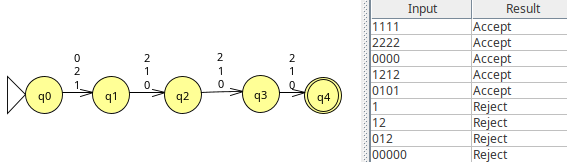
\includegraphics[width=0.9\textwidth]{imgs/163.png}
                                \caption{Diagrama de transiciones y validacion en JFLAP No. 163. }
                        \end{figure}
\end{minipage}
\end{center}

\begin{enumerate}
\setcounter{enumi}{163}
    \item Las palabras de $\Sigma_1$ con prefijo 20 y longitud 4.
    \begin{center}
        \begin{minipage}{0.45\textwidth}
            \begin{figure}[H]
    		\centering
    		
\includegraphics[width=1.2\textwidth]{imgs/ImgEma/AFN2L96.png}
            \end{figure}
        \end{minipage}
        \hfill
        \begin{minipage}{0.45\textwidth}
            \begin{center}
			\begin{tabular}{c|ccc}
			Estado actual & 0 & 1 & 2\\
			\hline
			$\rightarrow q0$ & $\emptyset$ & $\emptyset$ & $q1$\\
			$q1$ & $q2$ & $\emptyset$ & $\emptyset$\\
            $q2$ & $q3$ & $q3$ & $q3$\\
            $q3$ & $q4$ & $q4$ & $q4$\\
			$*q4$ & $\emptyset$ & $\emptyset$ & $\emptyset$\\
		      \end{tabular}
		      \end{center}
        \end{minipage}
        Se requiere una secuencia exacta de estados para los símbolos 2 y 0. Posteriormente, se consumen exactamente dos símbolos adicionales de cualquier tipo para garantizar que la longitud total de la cadena sea 4.
    \end{center}
\end{enumerate}

\newpage

\begin{enumerate}
\setcounter{enumi}{164}
\item*   Las palabras de $\Sigma_1$ cuya longitud es un múltiplo de 3.
\end{enumerate}

\begin{center}
\begin{minipage}{0.35\textwidth}
\begin{center}
    \textbf{Tabla de transiciones} \\
    \vspace{0.3cm}
    \begin{tabular}{c|ccc}
        Estado actual & 0 & 1 & 2 \\
        \hline
        $\rightarrow *q_0$ & $\{q_1\}$ & $\{q_1\}$ & $\{q_1\}$ \\
        $q_1$ & $\{q_2\}$ & $\{q_2\}$ & $\{q_2\}$ \\
        $q_2$ & $\{q_0\}$ & $\{q_0\}$ & $\{q_0\}$ \\
    \end{tabular}
\end{center}

				\textbf{Razonamiento:}\\
				Funciona como un contador cíclico módulo 3 ($q_0 \rightarrow q_1 \rightarrow q_2 \rightarrow q_0$). El estado inicial $q_0$ acepta la cadena vacía y los ciclos exactos. Cualquier cadena con longitud no divisible entre 3 se agota en los estados de tránsito ($q_1$ o $q_2$), siendo rechazada automáticamente.

\end{minipage}
\hfill
\begin{minipage}{0.55\textwidth}
\begin{figure}[H]

				\vspace{0.3cm}
                            \centering
                                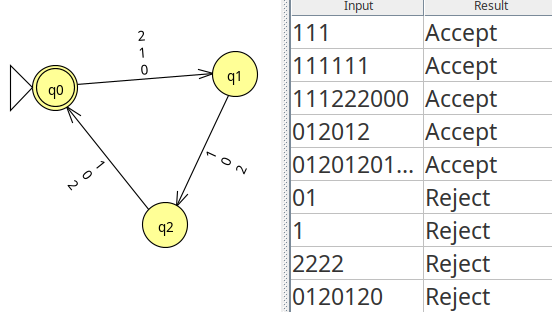
\includegraphics[width=0.9\textwidth]{imgs/165.png}
                                \caption{Diagrama de transiciones y validación en JFLAP No. 165}
                        \end{figure}



\end{minipage}
\end{center}
\vspace{0.5cm}

\begin{enumerate}
\setcounter{enumi}{165}
    \item Las palabras de $\Sigma_1$ que terminan con la cadena 00102.
    \begin{center}
        \begin{minipage}{0.45\textwidth}
            \begin{figure}[H]
    		\centering
    		
\includegraphics[width=1.2\textwidth]{imgs/ImgEma/AFN2L98.png}
            \end{figure}
        \end{minipage}
        \hfill
        \begin{minipage}{0.45\textwidth}
            \begin{center}
			\begin{tabular}{c|ccc}
			Estado actual & 0 & 1 & 2\\
			\hline
			$\rightarrow q0$ & $\{q0,q1\}$ & $q0$ & $q0$\\
			$q1$ & $q2$ & $\emptyset$ & $\emptyset$\\
            $q2$ & $\emptyset$ & $q3$ & $\emptyset$\\
            $q3$ & $q4$ & $\emptyset$ & $\emptyset$\\
			$q4$ & $\emptyset$ & $\emptyset$ & $q5$\\
            $*q5$ & $\emptyset$ & $\emptyset$ & $\emptyset$\\
		      \end{tabular}
		      \end{center}
        \end{minipage}
        El estado inicial posee un bucle que permite cualquier secuencia. El no determinismo ocurre cuando, al recibir un 0, el autómata decide si mantenerse en el bucle o iniciar la validación de la secuencia de cierre 00102.
    \end{center}
\end{enumerate}
\newpage
\begin{enumerate}
\setcounter{enumi}{166}
\item* Las palabras de $\Sigma_1$ cuya longitud es un múltiplo de 3.
\end{enumerate}

\begin{center}
\begin{minipage}{0.45\textwidth}
\begin{center}
    \textbf{Tabla de transiciones (AFND)} \\
    \vspace{0.3cm}
    \begin{tabular}{c|ccc}
        Estado actual & 0 & 1 & 2 \\
        \hline
        $\rightarrow q_0$ & $\{q_0, q_1\}$ & $\{q_0\}$ & $\{q_0\}$ \\
        $q_1$ & $\{q_2\}$ & $\emptyset$ & $\emptyset$ \\
        $q_2$ & $\emptyset$ & $\{q_3\}$ & $\emptyset$ \\
        $q_3$ & $\{q_4\}$ & $\emptyset$ & $\emptyset$ \\
        $q_4$ & $\{q_5\}$ & $\emptyset$ & $\emptyset$ \\
        $q_5$ & $\emptyset$ & $\{q_6\}$ & $\emptyset$ \\
        $*q_6$ & $\emptyset$ & $\emptyset$ & $\emptyset$ \\
    \end{tabular}
\end{center}

\vspace{0.3cm}
\textbf{Razonamiento:} \\
El estado inicial $q_0$ opera como un bucle infinito que procesa cualquier carácter. Al detectar un '0', el no determinismo (multiplicidad) entra en acción: un hilo se queda en $q_0$ esperando más texto, y otro hilo avanza a $q_1$ asumiendo que es el inicio de la secuencia final \textbf{001001}.
\end{minipage}
\hfill
\begin{minipage}{0.45\textwidth}
Esta ramificación lineal ($q_1 \rightarrow q_6$) exige los caracteres estrictos. Si la secuencia falla, ese hilo paralelo se destruye por omisión. Solo si los últimos seis caracteres coinciden, el hilo correspondiente sobrevivirá hasta el estado de aceptación $q_6$.
	\begin{figure}[H]
		\centering
		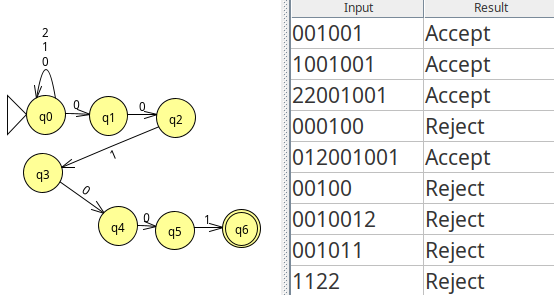
\includegraphics[width=0.9\textwidth]{imgs/167.png}
		\caption{Diagrama de trancisiones y validación en JFLAP No. 167.}
	\end{figure}	
\end{minipage}
\end{center}
\vspace{0.5cm}
\begin{enumerate}
\setcounter{enumi}{167}
    \item Las palabras de $\Sigma_2$ tales que el primer símbolo de la cadena es una letra y el segundo es un dígito.
    \begin{center}
        \begin{minipage}{0.45\textwidth}
            \begin{figure}[H]
    		\centering
    		
\includegraphics[width=1.2\textwidth]{imgs/ImgEma/AFN2L100.png}
            \end{figure}
        \end{minipage}
        \hfill
        \begin{minipage}{0.45\textwidth}
            \begin{center}
			\begin{tabular}{c|ccccc}
			Estado actual & a & b & c & 0 & 1\\
			\hline
			$\rightarrow q0$ & $q1$ & $q1$ & $q1$ & $\emptyset$ & $\emptyset$\\
			$q1$ & $\emptyset$ & $\emptyset$ & $\emptyset$ & $q2$ & $q2$\\
            $*q2$ & $q2$ & $q2$ & $q2$ & $q2$ & $q2$\\
		      \end{tabular}
		      \end{center}
        \end{minipage}
        Se valida que la primera transición provenga del subconjunto de letras $\{a, b, c\}$ y la segunda del subconjunto de dígitos $\{0, 1\}$. Si se cumplen estas condiciones, el autómata acepta cualquier símbolo posterior.
    \end{center}
\end{enumerate}

\newpage


\begin{enumerate}
\setcounter{enumi}{168}
\item Las palabras de $\Sigma_3$ que contienen la cadena aba
\end{enumerate}

\begin{center}
\begin{minipage}{0.45\textwidth}
\begin{center}
    \textbf{Tabla de transiciones (AFND)} \\
    \vspace{0.3cm}
    \begin{tabular}{c|cc}
        Estado actual & a & b \\
        \hline
        $\rightarrow q_0$ & $\{q_0, q_1\}$ & $\{q_0\}$ \\
        $q_1$ & $\emptyset$ & $\{q_2\}$ \\
        $q_2$ & $\{q_3\}$ & $\emptyset$ \\
        $*q_3$ & $\{q_3\}$ & $\{q_3\}$ \\
    \end{tabular}
\end{center}

\vspace{0.3cm}
\textbf{Razonamiento:} \\
El autómata emplea no determinismo en $q_0$ para evaluar el inicio de la subcadena. Al leer una 'a', la máquina se bifurca: un hilo permanece en $q_0$ consumiendo el prefijo basura, mientras otro avanza a $q_1$ para validar estrictamente la secuencia \textbf{aba} ($q_1 \rightarrow q_2 \rightarrow q_3$).
\end{minipage}
\hfill
\begin{minipage}{0.45\textwidth}
Una vez que el patrón se completa con éxito, el hilo alcanza el estado de aceptación $q_3$, el cual funciona como un sumidero de aceptación que absorbe cualquier combinación de 'a' y 'b' restante hasta el final de la cadena.
\begin{figure}[H]
	\centering
	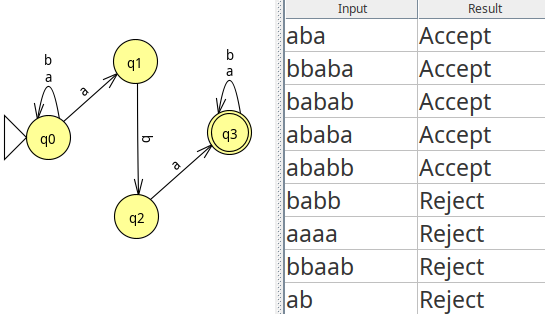
\includegraphics[width=0.9\textwidth]{imgs/169.png}
	\caption{Diagrama de transiciones y validación en JFLAP No.169}
\end{figure}
\end{minipage}
\end{center}
\vspace{0.5cm}
\begin{enumerate}
\setcounter{enumi}{169}
    \item Las palabras de $\Sigma_3$ que contienen la cadena abbbab.
    \begin{center}
        \begin{minipage}{0.45\textwidth}
            \begin{figure}[H]
    		\centering
    		
\includegraphics[width=1.2\textwidth]{imgs/ImgEma/AFN2L102.png}
            \end{figure}
        \end{minipage}
        \hfill
        \begin{minipage}{0.45\textwidth}
            \begin{center}
			\begin{tabular}{c|cc}
			Estado actual & a & b\\
			\hline
			$\rightarrow q0$ & $\{q0,q1\}$ & $q0$ \\
			$q1$ & $\emptyset$ & $q2$\\
            $q2$ & $\emptyset$ & $q3$\\
            $q3$ & $\emptyset$ & $q4$\\
            $q4$ & $q5$ & $\emptyset$\\
            $q5$ & $\emptyset$ & $q6$\\
            $*q6$ & $q6$ & $q6$\\
		      \end{tabular}
		      \end{center}
        \end{minipage}
        Se utiliza un bucle en el estado inicial para procesar símbolos arbitrarios hasta que se identifique el inicio de la cadena $abbbab$. Una vez encontrada y validada la subcadena, se acepta cualquier sufijo posterior.
    \end{center}
\end{enumerate}
\newpage
\begin{enumerate}
\setcounter{enumi}{170}
\item Las palabras de $\Sigma_3$ que contienen la cadena abbbab.
\end{enumerate}

\begin{center}
\begin{minipage}{0.45\textwidth}
\begin{center}
    \textbf{Tabla de transiciones (AFND)} \\
    \vspace{0.3cm}
    \begin{tabular}{c|cc}
        Estado actual & a & b \\
        \hline
        $\rightarrow q_0$ & $\{q_0, q_1\}$ & $\{q_0\}$ \\
        $q_1$ & $\{q_2\}$ & $\emptyset$ \\
        $q_2$ & $\emptyset$ & $\{q_3\}$ \\
        $q_3$ & $\emptyset$ & $\{q_4\}$ \\
        $q_4$ & $\emptyset$ & $\{q_5\}$ \\
        $q_5$ & $\{q_6\}$ & $\emptyset$ \\
        $*q_6$ & $\{q_6\}$ & $\{q_6\}$ \\
    \end{tabular}
\end{center}

\vspace{0.3cm}
\textbf{Razonamiento:} \\
El autómata utiliza no determinismo en $q_0$ para buscar el inicio del patrón en cualquier punto de la cadena. Al detectar la primera 'a', abre un hilo paralelo en $q_1$ para validar la secuencia exacta \textbf{aabbba} ($q_1 \rightarrow \dots \rightarrow q_6$).
\end{minipage}
\hfill
\begin{minipage}{0.45\textwidth}
Si el patrón falla en cualquier estado intermedio, ese hilo se destruye por omisión de transición ($\emptyset$). Si la secuencia se completa, el hilo sobrevive y alcanza el estado de aceptación $q_6$, el cual funciona como un sumidero que absorbe todo el texto restante validando la cadena
	\begin{figure}[H]
		\centering
		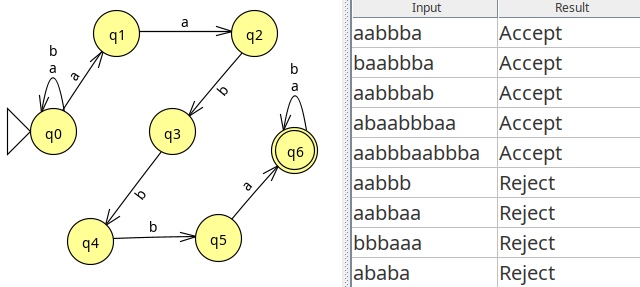
\includegraphics[width=0.9\textwidth]{imgs/171.png}
		\caption{Diagrama de transiciones y validación en JFLAP No. 171.}
	\end{figure}
\end{minipage}
\end{center}
\vspace{0.3cm}
\begin{enumerate}
\setcounter{enumi}{171}
    \item Las palabras de $\Sigma_3$ que inician con la cadena abbab.
    \begin{center}
        \begin{minipage}{0.45\textwidth}
            \begin{figure}[H]
    		\centering
    		
\includegraphics[width=1.2\textwidth]{imgs/ImgEma/AFN2L104.png}
            \end{figure}
        \end{minipage}
        \hfill
        \begin{minipage}{0.45\textwidth}
            \begin{center}
			\begin{tabular}{c|cc}
			Estado actual & a & b\\
			\hline
			$\rightarrow q0$ & $q1$ & $\emptyset$ \\
			$q1$ & $\emptyset$ & $q2$\\
            $q2$ & $\emptyset$ & $q3$\\
            $q3$ & $q5$ & $\emptyset$\\
            $q5$ & $\emptyset$ & $q4$\\
            $*q4$ & $\emptyset$ & $q6$\\
		      \end{tabular}
		      \end{center}
        \end{minipage}
        Ya que las palabras aceptadas por el AFN deben iniciar necesariamente con cadena abbab, por ende cualquier otro carácter posterior seria igualmente aceptado.
    \end{center}
\end{enumerate}

\newpage

\begin{enumerate}
\setcounter{enumi}{172}
\item Las palabras de $\Sigma_3$ que terminan con la cadena abaa.
\end{enumerate}

\begin{center}
\begin{minipage}{0.45\textwidth}
	\begin{center}
    \textbf{Tabla de transiciones (AFND)} \\
    \vspace{0.3cm}
    \begin{tabular}{c|cc}
        Estado actual & a & b \\
        \hline
        $\rightarrow q_0$ & $\{q_0, q_1\}$ & $\{q_0\}$ \\
        $q_1$ & $\emptyset$ & $\{q_2\}$ \\
        $q_2$ & $\{q_3\}$ & $\emptyset$ \\
        $q_3$ & $\{q_4\}$ & $\emptyset$ \\
        $*q_4$ & $\emptyset$ & $\emptyset$ \\
    \end{tabular}
\end{center}

\vspace{0.3cm}
\textbf{Razonamiento:} \\
Diseño optimizado para búsqueda de sufijos. El estado $q_0$ absorbe cualquier prefijo. Al leer una 'a', el no determinismo abre un hilo paralelo hacia $q_1$, asumiendo que es el inicio de la secuencia final \textbf{abaa}. Si la secuencia se interrumpe, ese hilo muere por omisión de transición. 

\end{minipage}
\hfill
\begin{minipage}{0.45\textwidth}
El estado de aceptación $q_4$ carece intencionalmente de salidas; cualquier carácter que ingrese después de completar la secuencia destruirá el hilo, garantizando que la cadena termine estrictamente con el patrón solicitado.
	\begin{figure}[H]
		\centering
		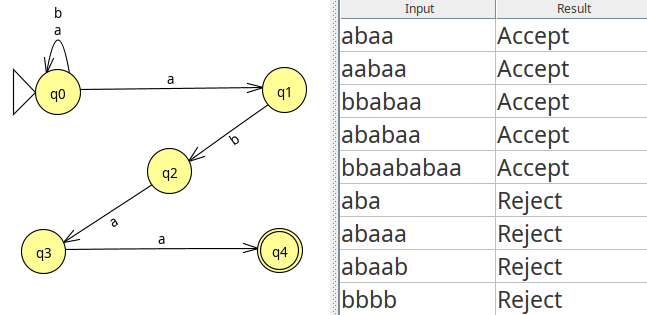
\includegraphics[width=0.9\textwidth]{imgs/173.png}
		\caption{Diagrama de transiciones y valdación en JFLAP No. 173.}
	\end{figure}
\end{minipage}
\end{center}
\vspace{0.5cm}

\begin{enumerate}
\setcounter{enumi}{173}
    \item Las palabras de $\Sigma_1$ que incluyen la subcadena 1101001.
    \begin{center}
        \begin{minipage}{0.45\textwidth}
            \begin{figure}[H]
    		\centering
    		
\includegraphics[width=1.2\textwidth]{imgs/ImgEma/AFN2L106.png}
            \end{figure}
        \end{minipage}
        \hfill
        \begin{minipage}{0.45\textwidth}
            \begin{center}
			\begin{tabular}{c|ccc}
			Estado actual & 0 & 1 & 2\\
			\hline
			$\rightarrow q0$ & $q0$ & $\{q0,q1\}$ & $q0$\\
			$q1$ & $\emptyset$ & $q2$ & $\emptyset$\\
            $q2$ & $q3$ & $\emptyset$ & $\emptyset$\\
            $q3$ & $\emptyset$ & $q4$ & $\emptyset$\\
			$q4$ & $q5$ & $\emptyset$ & $\emptyset$\\
            $q5$ & $q6$ & $\emptyset$ & $\emptyset$\\
            $q6$ & $\emptyset$ & $q7$ & $\emptyset$\\
            $*q7$ & $q7$ & $q7$ & $q7$\\
		      \end{tabular}
		      \end{center}
        \end{minipage}
        El estado inicial y final posee un bucle que permite cualquier secuencia. El no determinismo ocurre cuando, al recibir un 1, el autómata decide si mantenerse en el bucle o iniciar la validación de la subcadena de cierre 1101001.
    \end{center}
\end{enumerate}
\newpage
\begin{enumerate}
\setcounter{enumi}{174}
\item Las palabras de $\Sigma_1$ que incluyen al menos una vez la subcadena 0101 y
al menos una vez la subcadena 021.
\end{enumerate}

\begin{center}
\begin{minipage}{0.45\textwidth}
	\begin{center}
    \textbf{Tabla de transiciones (AFND)} \\
    \vspace{0.3cm}
    \begin{tabular}{c|ccc}
        Estado actual & 0 & 1 & 2 \\
        \hline
        $\rightarrow q_0$ & $\{q_0, q_1, q_7\}$ & $\{q_0\}$ & $\{q_0\}$ \\
        $q_1$ & $\emptyset$ & $\{q_2\}$ & $\emptyset$ \\
        $q_2$ & $\{q_3\}$ & $\emptyset$ & $\emptyset$ \\
        $q_3$ & $\emptyset$ & $\{q_4\}$ & $\emptyset$ \\
        $q_4$ & $\{q_4, q_5\}$ & $\{q_4\}$ & $\{q_4\}$ \\
        $q_5$ & $\emptyset$ & $\emptyset$ & $\{q_6\}$ \\
        $q_6$ & $\emptyset$ & $\{q_{13}\}$ & $\emptyset$ \\
        $q_7$ & $\emptyset$ & $\emptyset$ & $\{q_8\}$ \\
        $q_8$ & $\emptyset$ & $\{q_9\}$ & $\emptyset$ \\
        $q_9$ & $\{q_9, q_{10}\}$ & $\{q_9\}$ & $\{q_9\}$ \\
        $q_{10}$ & $\emptyset$ & $\{q_{11}\}$ & $\emptyset$ \\
        $q_{11}$ & $\{q_{12}\}$ & $\emptyset$ & $\emptyset$ \\
        $q_{12}$ & $\emptyset$ & $\{q_{13}\}$ & $\emptyset$ \\
        $*q_{13}$ & $\{q_{13}\}$ & $\{q_{13}\}$ & $\{q_{13}\}$ \\
    \end{tabular}
\end{center}

\vspace{0.3cm}
\end{minipage}
\hfill
\begin{minipage}{0.45\textwidth}
\textbf{Razonamiento:} \\
El autómata emplea no determinismo en $q_0$ para procesar tres escenarios simultáneos cada vez que lee un '0': mantenerse consumiendo ruido ($q_0$), intentar validar primero la secuencia \textbf{0101} ($q_1 \rightarrow q_4$), o intentar validar primero la secuencia \textbf{021} ($q_7 \rightarrow q_9$). Los estados intermedios $q_4$ y $q_9$ actúan como pivotes de espera; una vez hallado el primer patrón, retienen el hilo de ejecución iterando sobre cualquier carácter hasta detectar el inicio del segundo. El estado de aceptación $q_{13}$ solo es alcanzable si un mismo hilo logra completar ambas búsquedas en el orden que sea, absorbiendo el resto de la cadena.
\end{minipage}

\begin{minipage}{0.45\textwidth}
	\begin{figure}[H]
		\centering
		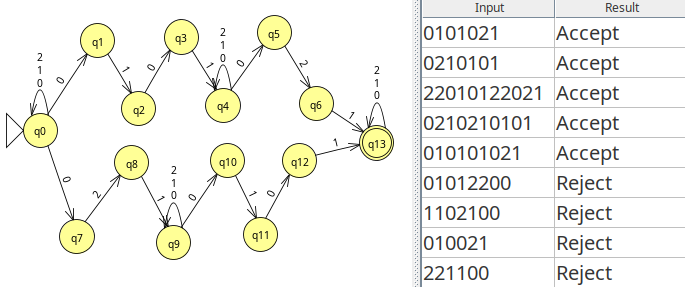
\includegraphics[width=0.9\textwidth]{imgs/175.png}
		\caption{Diagrama de transiciones y validación No. 173.}
	\end{figure}
\end{minipage}
\end{center}
\vspace{0.3cm}

\begin{enumerate}
\setcounter{enumi}{175}
    \item Las palabras de $\Sigma_2$ que incluyen al menos una vez la subcadena abbcb y al menos una vez la subcadena cbaabb, asumiendo que no se pueden traslapar; así, cadenas similares a abbcbaabb no están en el lenguaje.
    \begin{center}
        \begin{minipage}{0.45\textwidth}
            \begin{figure}[H]
    		\centering
    		
\includegraphics[width=1\textwidth]{imgs/ImgEma/AFN2L108.png}
            \end{figure}
        \end{minipage}
        \hfill
        \begin{minipage}{0.45\textwidth}
            Se presenta este AFN como solución parcial, pues se debe de ramificar el proceso, $i.e.$, una rama busca primero abbcb y luego cbaabb, mientras que la otra busca el orden inverso, cabe aclarar que la herramienta JFLAP no permite ramificar correctamente, pues se marca error en cierto momento si se llegan a repetir salidas mas de 2 veces.
        \end{minipage}
    \end{center}
\end{enumerate}

\newpage 
\begin{enumerate}
\setcounter{enumi}{176}
\item Las palabras de $\Sigma_2$ que incluyen al menos una vez la subcadena abbcb y al menos una vez la subcadena cbaabb, asumiendo que sí se pueden traslapar.
\end{enumerate}

\begin{center}   

    \textbf{Tabla de transiciones (AFND con traslape)} \\
    \vspace{0.3cm}
    \begin{tabular}{c|ccccc}
        Estado & a & b & c & 0 & 1 \\
        \hline
        $\rightarrow q_0$ & $\{q_0, q_1\}$ & $\{q_0\}$ & $\{q_0, q_6\}$ & $\{q_0\}$ & $\{q_0\}$ \\
        $q_1$ & $\emptyset$ & $\{q_2\}$ & $\emptyset$ & $\emptyset$ & $\emptyset$ \\
        $q_2$ & $\emptyset$ & $\{q_3\}$ & $\emptyset$ & $\emptyset$ & $\emptyset$ \\
        $q_3$ & $\emptyset$ & $\emptyset$ & $\{q_4\}$ & $\emptyset$ & $\emptyset$ \\
        $q_4$ & $\emptyset$ & $\{q_5, q_{13}\}$ & $\emptyset$ & $\emptyset$ & $\emptyset$ \\
        $q_5$ & $\{q_5\}$ & $\{q_5\}$ & $\{q_5, q_{12}\}$ & $\{q_5\}$ & $\{q_5\}$ \\
        $q_6$ & $\emptyset$ & $\{q_7\}$ & $\emptyset$ & $\emptyset$ & $\emptyset$ \\
        $q_7$ & $\{q_8\}$ & $\emptyset$ & $\emptyset$ & $\emptyset$ & $\emptyset$ \\
        $q_8$ & $\{q_9\}$ & $\emptyset$ & $\emptyset$ & $\emptyset$ & $\emptyset$ \\
        $q_9$ & $\emptyset$ & $\{q_{10}\}$ & $\emptyset$ & $\emptyset$ & $\emptyset$ \\
        $q_{10}$ & $\emptyset$ & $\{q_{11}, q_{19}\}$ & $\emptyset$ & $\emptyset$ & $\emptyset$ \\
        $q_{11}$ & $\{q_{11}, q_{17}\}$ & $\{q_{11}\}$ & $\{q_{11}\}$ & $\{q_{11}\}$ & $\{q_{11}\}$ \\
        $q_{12}$ & $\emptyset$ & $\{q_{13}\}$ & $\emptyset$ & $\emptyset$ & $\emptyset$ \\
        $q_{13}$ & $\{q_{14}\}$ & $\emptyset$ & $\emptyset$ & $\emptyset$ & $\emptyset$ \\
        $q_{14}$ & $\{q_{15}\}$ & $\emptyset$ & $\emptyset$ & $\emptyset$ & $\emptyset$ \\
        $q_{15}$ & $\emptyset$ & $\{q_{16}\}$ & $\emptyset$ & $\emptyset$ & $\emptyset$ \\
        $q_{16}$ & $\emptyset$ & $\{q_{21}\}$ & $\emptyset$ & $\emptyset$ & $\emptyset$ \\
        $q_{17}$ & $\emptyset$ & $\{q_{18}\}$ & $\emptyset$ & $\emptyset$ & $\emptyset$ \\
        $q_{18}$ & $\emptyset$ & $\{q_{19}\}$ & $\emptyset$ & $\emptyset$ & $\emptyset$ \\
        $q_{19}$ & $\emptyset$ & $\emptyset$ & $\{q_{20}\}$ & $\emptyset$ & $\emptyset$ \\
        $q_{20}$ & $\emptyset$ & $\{q_{21}\}$ & $\emptyset$ & $\emptyset$ & $\emptyset$ \\
        $*q_{21}$ & $\{q_{21}\}$ & $\{q_{21}\}$ & $\{q_{21}\}$ & $\{q_{21}\}$ & $\{q_{21}\}$ \\
    \end{tabular}





\begin{minipage}{0.35\textwidth}
\textbf{Razonamiento:} \\
El autómata emplea bifurcación paralela desde $q_0$ para buscar \textbf{abbcb} ($q_1$) o \textbf{cbaabb} ($q_6$). La optimización radica en la gestión explícita del traslape sin usar transiciones $\epsilon$. 

\vspace{0.3cm}
Al completar \textbf{abbcb} (estado $q_4 \rightarrow \text{leyendo } b$), el hilo se bifurca en dos: a $q_5$ (para esperar pasivamente la segunda cadena) y a $q_{13}$. El envío a $q_{13}$ asume que el sufijo recién leído \textbf{cb} es simultáneamente el prefijo de la segunda cadena, requiriendo solo \textbf{aabb} para alcanzar la aceptación.

\end{minipage}
\hfill
\begin{minipage}{0.55\textwidth}
La misma lógica inversa aplica al completar \textbf{cbaabb} ($q_{10} \rightarrow \text{leyendo } b$): se bifurca a $q_{11}$ (espera pasiva) y a $q_{19}$, asumiendo que el sufijo \textbf{abb} es el inicio de la primera cadena, requiriendo solo \textbf{cb} para finalizar. $q_{21}$ actúa como sumidero de éxito absoluto.
	\begin{figure}[H]
		\centering
		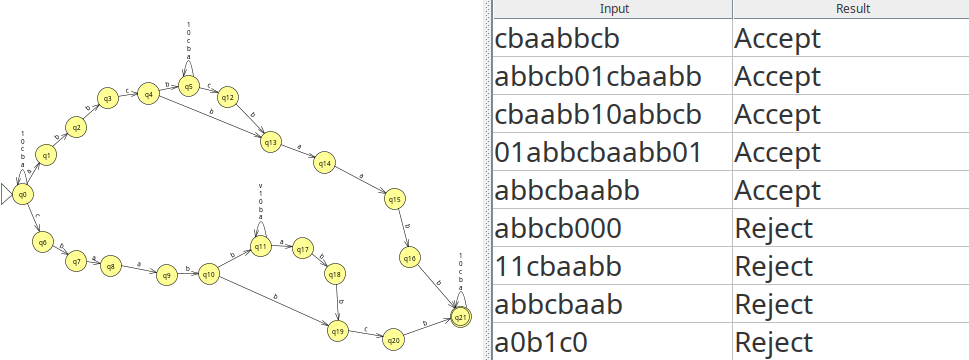
\includegraphics[width=0.9\textwidth]{imgs/177.png}
		\caption{Diagrama de transiciones y validación No. 177.}
	\end{figure}
\end{minipage}
\end{center}
\newpage

\begin{enumerate}
\setcounter{enumi}{177}
    \item Las palabras de $\Sigma_1$ que contienen exactamente tres veces la subcadena 01.
    \begin{center}
        \begin{minipage}{0.45\textwidth}
            \begin{figure}[H]
    		\centering
    		
\includegraphics[width=1.2\textwidth]{imgs/ImgEma/AFN2L110.png}
            \end{figure}
        \end{minipage}
        \hfill
        \begin{minipage}{0.45\textwidth}
            \begin{center}
            \begin{tabular}{c|ccc}
            Estado actual & 0 & 1 & 2\\
            \hline
            $\rightarrow q0$ & $q1$ & $q0$ & $q0$ \\
            $q1$ & $q1$ & $q2$ & $q0$\\
            $q2$ & $q3$ & $q2$ & $q2$\\
            $q3$ & $q3$ & $q4$ & $q2$\\
            $q4$ & $q5$ & $q4$ & $q4$\\
            $q5$ & $q5$ & $*q6$ & $q4$\\
            $*q6$ & $q7$ & $q6$ & $q6$\\
            $q7$ & $q7$ & $\emptyset$ & $q6$\\
            \end{tabular}
            \end{center}
        \end{minipage}
        Se requiere un conteo estricto. Los estados pares indican cuántas veces se ha completado la subcadena, mientras que los impares son estados de espera tras recibir un 0.
    \end{center}
\end{enumerate}


\vspace{0.3cm}
\begin{enumerate}
\setcounter{enumi}{178}
\item Las palabras de $\Sigma_1$ que contienen exactamente tres veces la subcadena 01002.
\end{enumerate}
\begin{minipage}{0.45\textwidth}
\begin{center}
    \textbf{Tabla de transiciones (AFND Contador Estricto)} \\
    \vspace{0.3cm}
    \begin{tabular}{c|ccc}
        Estado & 0 & 1 & 2 \\
	\hline
        $\rightarrow q_0$ & $\{q_1\}$ & $\{q_0\}$ & $\{q_0\}$ \\
        $q_1$ & $\{q_1\}$ & $\{q_2\}$ & $\{q_0\}$ \\
        $q_2$ & $\{q_3\}$ & $\{q_0\}$ & $\{q_0\}$ \\
        $q_3$ & $\{q_4\}$ & $\{q_2\}$ & $\{q_0\}$ \\
        $q_4$ & $\{q_1\}$ & $\{q_0\}$ & $\{q_5\}$ \\
        $q_5$ & $\{q_6\}$ & $\{q_5\}$ & $\{q_5\}$ \\
        $q_6$ & $\{q_6\}$ & $\{q_7\}$ & $\{q_5\}$ \\
        $q_7$ & $\{q_8\}$ & $\{q_5\}$ & $\{q_5\}$ \\
        $q_8$ & $\{q_9\}$ & $\{q_7\}$ & $\{q_5\}$ \\
        $q_9$ & $\{q_6\}$ & $\{q_5\}$ & $\{q_{10}\}$ \\
        $q_{10}$ & $\{q_{11}\}$ & $\{q_{10}\}$ & $\{q_{10}\}$ \\
        $q_{11}$ & $\{q_{11}\}$ & $\{q_{12}\}$ & $\{q_{10}\}$ \\
        $q_{12}$ & $\{q_{13}\}$ & $\{q_{10}\}$ & $\{q_{10}\}$ \\
        $q_{13}$ & $\{q_{14}\}$ & $\{q_{12}\}$ & $\{q_{10}\}$ \\
        $q_{14}$ & $\{q_{11}\}$ & $\{q_{10}\}$ & $\{q_{15}\}$ \\
        $*q_{15}$ & $\{q_{16}\}$ & $\{q_{15}\}$ & $\{q_{15}\}$ \\
        $*q_{16}$ & $\{q_{16}\}$ & $\{q_{17}\}$ & $\{q_{15}\}$ \\
        $*q_{17}$ & $\{q_{18}\}$ & $\{q_{15}\}$ & $\{q_{15}\}$ \\
        $*q_{18}$ & $\{q_{19}\}$ & $\{q_{17}\}$ & $\{q_{15}\}$ \\
        $*q_{19}$ & $\{q_{16}\}$ & $\{q_{15}\}$ & $\emptyset$ \\
    \end{tabular}
\end{center}
\end{minipage}
\hfill
\begin{minipage}{0.45\textwidth}
\textbf{Razonamiento:} \\
El autómata consta de cuatro bloques secuenciales que rastrean la subcadena \textbf{01002}. Cada bloque incorpora rutas de retroceso precisas (ej. $q_3 \xrightarrow{1} q_2$) para evitar perder progreso si el patrón falla parcialmente. Al completarse la secuencia (transición con '2'), el hilo avanza al siguiente bloque. Al completarse por tercera vez, ingresa al Bloque 3, donde todos los estados son de aceptación, ya que el requisito de "tres veces" está cumplido independientemente del ruido posterior. El control estricto recae en el estado $q_{19}$: si se está a punto de completar una cuarta aparición y se lee un '2', la transición es nula ($\emptyset$), destruyendo el hilo y rechazando la cadena por exceso de ocurrencias.
\end{minipage}
\begin{center}

\begin{minipage}{0.75\textwidth}
\begin{figure}[H]
                \centering
                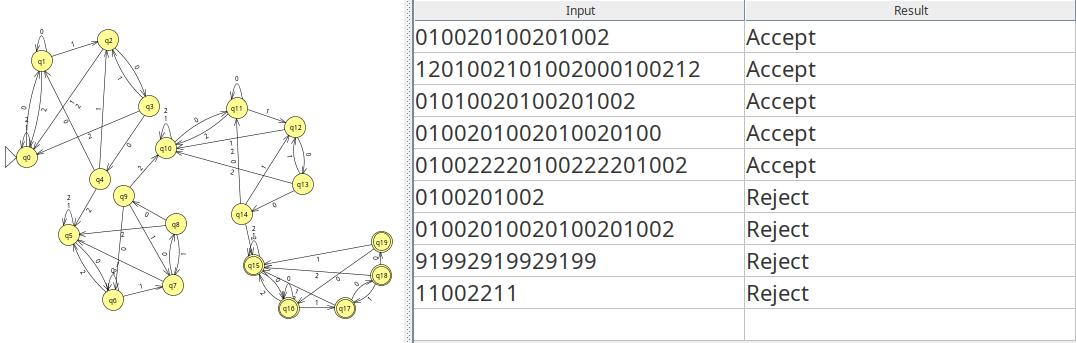
\includegraphics[width=0.9\textwidth]{imgs/179.png}
                \caption{Diagrama de transiciones y validación No. 179.}
        \end{figure}
\end{minipage}
\end{center}

\begin{enumerate}
\setcounter{enumi}{179}
    \item Las palabras de $\Sigma_1$ que contienen dos veces la subcadena 010, asumiendo que no se pueden traslapar; es decir, que 01010 no está en el lenguaje, mientras que 010010 sí pertenece.
    \begin{center}
        \begin{minipage}{0.45\textwidth}
            \begin{figure}[H]
    		\centering
    		
\includegraphics[width=1.2\textwidth]{imgs/ImgEma/AFN2L112.png}
            \end{figure}
        \end{minipage}
        \hfill
        \begin{minipage}{0.45\textwidth}
            \begin{center}
            \begin{tabular}{c|ccc}
            Estado actual & 0 & 1 & 2\\
            \hline
            $\rightarrow q0$ & $\{q0, q1\}$ & $q0$ & $q0$ \\
            $q1$ & $\emptyset$ & $q2$ & $\emptyset$\\
            $q2$ & $q3$ & $\emptyset$ & $\emptyset$\\
            $q3$ & $\{q3, q4\}$ & $q3$ & $q3$\\
            $q4$ & $\emptyset$ & $q5$ & $\emptyset$\\
            $q5$ & $*q6$ & $\emptyset$ & $\emptyset$\\
            $*q6$ & $q6$ & $q6$ & $q6$\\
            \end{tabular}
            \end{center}
        \end{minipage}
        Similar al ejercicio 110, pero una vez que se completa el primer 010, el sistema debe ignorar ese último 0 para evitar el traslape y empezar a buscar el segundo bloque desde cero lo cual nos obliga a usar una transición extra.
    \end{center}
\end{enumerate}

\newpage
\begin{enumerate}
\setcounter{enumi}{180}
\item Las palabras de $\Sigma_1$ que contienen dos veces la subcadena 010, asumiendo que sí se pueden traslapar. 
\end{enumerate}

\begin{center}
\begin{minipage}{0.45\textwidth}
\begin{center}
    \textbf{Tabla de transiciones (AFND con traslape)} \\
    \vspace{0.3cm}
    \begin{tabular}{c|ccc}
        Estado & 0 & 1 & 2 \\
        \hline
        $\rightarrow q_0$ & $\{q_0, q_1\}$ & $\{q_0\}$ & $\{q_0\}$ \\
        $q_1$ & $\emptyset$ & $\{q_2\}$ & $\emptyset$ \\
        $q_2$ & $\{q_3, q_4\}$ & $\emptyset$ & $\emptyset$ \\
        $q_3$ & $\emptyset$ & $\{q_6\}$ & $\emptyset$ \\
        $q_4$ & $\{q_4, q_5\}$ & $\{q_4\}$ & $\{q_4\}$ \\
        $q_5$ & $\emptyset$ & $\{q_6\}$ & $\emptyset$ \\
        $q_6$ & $\{q_7\}$ & $\emptyset$ & $\emptyset$ \\
        $*q_7$ & $\{q_7\}$ & $\{q_7\}$ & $\{q_7\}$ \\
    \end{tabular}
\end{center}

\vspace{0.3cm}
\textbf{Razonamiento:} \\
Al completar la primera subcadena en $q_2$, la lectura del último '0' bifurca la ejecución. El hilo en $q_3$ evalúa el traslape inmediato, requiriendo solo \textbf{10} para aceptar (ej. \textbf{01010}). 

\end{minipage}
\hfill
\begin{minipage}{0.45\textwidth}

Simultáneamente, el hilo en $q_4$ absorbe texto basura hasta validar una segunda aparición independiente. Ambas rutas convergen hacia el sumidero de aceptación absoluta $q_7$.

\begin{figure}[H]
                \centering
                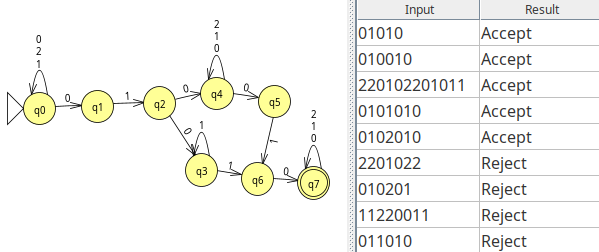
\includegraphics[width=0.9\textwidth]{imgs/181.png}
                \caption{Diagrama de transiciones y validación No. 181.}
        \end{figure}
\end{minipage}
\end{center}
\vspace{0.5cm}
\begin{enumerate}
\setcounter{enumi}{181}
    \item $L=\{w\in\Sigma_3^*:w=a^nb^m,n,m\in\mathbb{N}\}.$
    \begin{center}
        \begin{minipage}{0.45\textwidth}
            \begin{figure}[H]
    		\centering
    		
\includegraphics[width=1.2\textwidth]{imgs/ImgEma/AFN2L114.png}
            \end{figure}
        \end{minipage}
        \hfill
        \begin{minipage}{0.45\textwidth}
            \begin{center}
            \begin{tabular}{c|cc}
            Estado actual & a & b\\
            \hline
            $\rightarrow q0$ & $q1$ & $\emptyset$ \\
            $q1$ & $q1$ & $q2$\\
            $*q2$ & $\emptyset$ & $q2$\\
            \end{tabular}
            \end{center}
        \end{minipage}
        Siendo $\mathbb{N} = \{1, 2, 3, \dots\}$, la cadena debe tener al menos una a y al menos una b, $i.e:\ a^+b^+$, ademas que el orden importa, por lo que si inicia con b o finaliza con a, la palabra no es aceptada.
    \end{center}
\end{enumerate}

\newpage
\begin{enumerate}
\setcounter{enumi}{182}
\item $L = \{w \in \Sigma_2 : w = (abc)^n, n \in \mathbb{N}\}$.
\end{enumerate}

\begin{center}
\begin{minipage}{0.45\textwidth}

\begin{center}
    \textbf{Tabla de transiciones (AFND)} \\
    \vspace{0.3cm}
    \begin{tabular}{c|ccccc}
        Estado & a & b & c & 0 & 1 \\
        \hline
        $\rightarrow *q_0$ & $\{q_1\}$ & $\emptyset$ & $\emptyset$ & $\emptyset$ & $\emptyset$ \\
        $q_1$ & $\emptyset$ & $\{q_2\}$ & $\emptyset$ & $\emptyset$ & $\emptyset$ \\
        $q_2$ & $\emptyset$ & $\emptyset$ & $\{q_0\}$ & $\emptyset$ & $\emptyset$ \\
    \end{tabular}
\end{center}

\vspace{0.3cm}
\textbf{Razonamiento:} \\
Opera como un ciclo estricto ($q_0 \xrightarrow{a} q_1 \xrightarrow{b} q_2 \xrightarrow{c} q_0$) diseñado para validar la secuencia exacta \textbf{abc}. El estado inicial $q_0$ es de aceptación para admitir la cadena vacía ($n=0$) y las repeticiones completas del 
\end{minipage}
\hfill
\begin{minipage}{0.45\textwidth}

ciclo. Cualquier desviación del patrón (orden incorrecto o la intrusión de los símbolos '0' y '1') carece de salida definida ($\emptyset$), destruyendo el hilo inmediatamente y rechazando la cadena.
\begin{figure}[H]
                \centering
                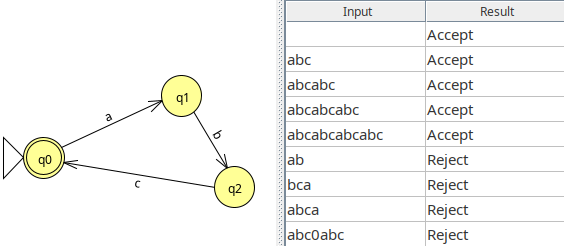
\includegraphics[width=0.9\textwidth]{imgs/183.png}
                \caption{Diagrama de transiciones y validación No. 183.}
        \end{figure}
\end{minipage}
\end{center}
\vspace{0.4cm}
\begin{enumerate}
\setcounter{enumi}{183}
    \item $L=\{w\in\Sigma_2:w=a^nb^mc^{n+1},n,m\in\mathbb{N}\}.$
    \begin{center}
        Este lenguaje no es regular. Debido a que el número de letras c depende directamente del número de letras a ($n$ y $n+1$), es decir, se requiere memoria infinita para su reconocimiento. Por lo tanto, no es posible realizar un AFN, ya que este lenguaje pertenece a la categoría de los Lenguajes Libres de Contexto (requiere un Autómata de Pila).
    \end{center}
\end{enumerate}

\begin{enumerate}
\setcounter{enumi}{184}
\item $L = \{w \in \Sigma_3 : w = a^n b^m a^p b^q, m, n, p, q \in \mathbb{N}\}$.
\end{enumerate}

\begin{center}
\begin{minipage}{0.45\textwidth}
	\begin{center}
    \textbf{Tabla de transiciones (AFND)} \\
    \vspace{0.3cm}
    \begin{tabular}{c|ccc}
        Estado & a & b & c \\
        \hline
        $\rightarrow q_0$ & $\{q_1\}$ & $\emptyset$ & $\emptyset$ \\
        $q_1$ & $\{q_1\}$ & $\{q_2\}$ & $\emptyset$ \\
        $q_2$ & $\{q_3\}$ & $\{q_2\}$ & $\emptyset$ \\
        $q_3$ & $\{q_3\}$ & $\{q_4\}$ & $\emptyset$ \\
        $*q_4$ & $\emptyset$ & $\{q_4\}$ & $\emptyset$ \\
    \end{tabular}
\end{center}

\vspace{0.3cm}
\textbf{Razonamiento:} \\
El diseño impone una progresión secuencial estricta para validar los cuatro bloques de la expresión ($a \rightarrow b \rightarrow a \rightarrow b$). Cada cambio de símbolo avanza la máquina a la siguiente fase ($q_1 \xrightarrow{b} q_2 \xrightarrow{a} q_3 \xrightarrow{b} q_4$). Al definir $q_4$ como el único estado de 
\end{minipage}
\hfill
\begin{minipage}{0.45\textwidth}
aceptación, se garantiza matemáticamente que los cuatro bloques existan (mínimo una iteración por bloque). La intrusión de un símbolo 'c', o intentar leer una 'a' después de haber entrado al último bloque de 'b's, redirige a $\emptyset$, destruyendo el hilo y rechazando la cadena instantáneamente.

\begin{figure}[H]
                \centering
                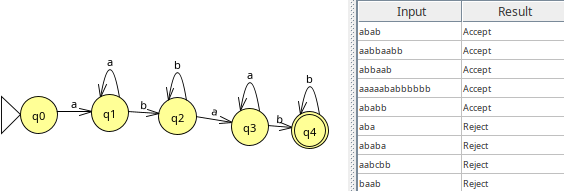
\includegraphics[width=0.9\textwidth]{imgs/185.png}
                \caption{Diagrama de transiciones y validación No. 185.}
        \end{figure}

\end{minipage}
\end{center}

\newpage
\begin{enumerate}
\setcounter{enumi}{185}
    \item $L=\{w\in\Sigma_3:w=axabya,x,y\in\Sigma_3^*\}.$
    \begin{center}
        \begin{minipage}{0.45\textwidth}
            \begin{figure}[H]
    		\centering
    		
\includegraphics[width=1.2\textwidth]{imgs/ImgEma/AFN2L118.png}
            \end{figure}
        \end{minipage}
        \hfill
        \begin{minipage}{0.45\textwidth}
            \begin{center}
            \begin{tabular}{c|cc}
            Estado actual & a & b\\
            \hline
            $\rightarrow q0$ & $q1$ & $\emptyset$ \\
            $q1$ & $\{q1, q2\}$ & $q1$\\
            $q2$ & $\emptyset$ & $q3$\\
            $q3$ & $\{q3, q4\}$ & $q3$\\
            $*q4$ & $\emptyset$ & $\emptyset$\\
            \end{tabular}
            \end{center}
        \end{minipage}
        La cadena debe seguir el patrón fijo: comienza con a, sigue cualquier cosa ($x$), luego a, luego b, sigue cualquier cosa ($y$) y termina con a, ya que tenemos la condición de $x,y\in\Sigma_3^*$, esto nos indica que $x$ y $y$, pueden ser $\lambda$ o hasta una palabra distinta.
    \end{center}
\end{enumerate}

\vspace{0.5cm}
\begin{enumerate}
\setcounter{enumi}{186}
\item Las palabras de $\Sigma_3$ tales que después de cada subcadena $aa$ aparece una $b$.
\end{enumerate}

\begin{center}
\begin{minipage}{0.45\textwidth}
\begin{center}
    \textbf{Tabla de transiciones (AFND)} \\
    \vspace{0.3cm}
    \begin{tabular}{c|cc}
        Estado actual & a & b \\
        \hline
        $\rightarrow *q_0$ & $\{q_1\}$ & $\{q_0\}$ \\
        $*q_1$ & $\{q_2\}$ & $\{q_0\}$ \\
        $q_2$ & $\emptyset$ & $\{q_0\}$ \\
    \end{tabular}
\end{center}

\vspace{0.3cm}
\textbf{Razonamiento:} \\
La máquina evalúa secuencias restrictivas de forma lineal. El estado $q_0$ procesa texto seguro. Al leer una 'a', avanza a $q_1$. Si lee una segunda 'a', entra al estado crítico $q_2$, el cual no es de aceptación. En este punto, la regla exige una 'b' para validar la subcadena; si se lee, el hilo regresa a la seguridad de $q_0$. Si por el contrario se in-
\end{minipage}
\hfill
\begin{minipage}{0.45\textwidth}

tenta leer una tercera 'a' (formando la secuencia prohibida \textbf{aaa}), la transición nula ($\emptyset$) destruye el hilo de ejecución. Adicionalmente, cualquier cadena que termine exactamente en \textbf{aa} quedará atrapada en $q_2$, siendo rechazada por carecer de la 'b' final exigida.
\begin{figure}[H]
                \centering
                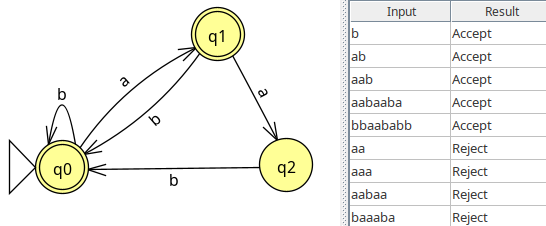
\includegraphics[width=0.9\textwidth]{imgs/187.png}
                \caption{Diagrama de transiciones y validación No. 187.}
        \end{figure}
\end{minipage}
\end{center}

\newpage
\begin{enumerate}
\setcounter{enumi}{187}
    \item Las palabras de $\Sigma_1$ tales que el primer carácter y el último son distintos.
    \begin{center}
        \begin{minipage}{0.45\textwidth}
            \begin{figure}[H]
    		\centering
    		
\includegraphics[width=1.2\textwidth]{imgs/ImgEma/AFN2L120.png}
            \end{figure}
        \end{minipage}
        \hfill
        \begin{minipage}{0.45\textwidth}
            \begin{center}
            \begin{tabular}{c|ccc}
            Estado actual & 0 & 1 & 2\\
            \hline
            $\rightarrow q0$ & $q1$ & $q2$ & $q3$ \\
            $q1$ & $q1$ & $\{q1, q4\}$ & $\{q1, q4\}$\\
            $q2$ & $\{q2, q4\}$ & $q2$ & $\{q2, q4\}$\\
            $q3$ & $\{q3, q4\}$ & $\{q3, q4\}$ & $q3$\\
            $*q4$ & $\emptyset$ & $\emptyset$ & $\emptyset$\\
            \end{tabular}
            \end{center}
        \end{minipage}
        Se deben crean tres rutas paralelas dependiendo del primer símbolo recibido, gracias a los AFN esto es capaz de traslapar transiciones entre si.
    \end{center}
\end{enumerate}

\begin{enumerate}
\setcounter{enumi}{188}
\item Encuentre un autómata finito no determinista con lenguaje $\Sigma=\{0, 1\}$ que identifique las palabras que contienen la cadena 00101 o la cadena 00110. Realice el diagrama de transiciones de la palabra 1001011.
\end{enumerate}

\begin{center}
\begin{minipage}{0.45\textwidth}
\begin{center}
    \textbf{Tabla de transiciones (AFND con prefijo común)} \\
    \vspace{0.3cm}
    \begin{tabular}{c|cc}
        Estado & 0 & 1 \\
        \hline
        $\rightarrow q_0$ & $\{q_0, q_1\}$ & $\{q_0\}$ \\
        $q_1$ & $\{q_2\}$ & $\emptyset$ \\
        $q_2$ & $\emptyset$ & $\{q_3\}$ \\
        $q_3$ & $\{q_4\}$ & $\{q_5\}$ \\
        $q_4$ & $\emptyset$ & $\{q_6\}$ \\
        $q_5$ & $\{q_6\}$ & $\emptyset$ \\
        $*q_6$ & $\{q_6\}$ & $\{q_6\}$ \\
    \end{tabular}
\end{center}
\vspace{0.3cm}
\end{minipage}
\hfill
\begin{minipage}{0.45\textwidth}

\vspace{0.3cm}
\textbf{Diagrama de transiciones (Traza de conjuntos) para $w = 1001011$:} \\
La ejecución de un AFND se demuestra evaluando los estados activos simultáneos paso a paso:
\begin{itemize}[noitemsep, label=-]
    \item \textbf{Inicio:} $\{q_0\}$
    \item Leer \textbf{1}: $\{q_0\}$
    \item Leer \textbf{0}: $\{q_0, q_1\}$
    \item Leer \textbf{0}: $\{q_0, q_1, q_2\}$
    \item Leer \textbf{1}: $\{q_0, q_3\}$
    \item Leer \textbf{0}: $\{q_0, q_1, q_4\}$
    \item Leer \textbf{1}: $\{q_0, q_6\}$ \textit{(El patrón 00101 se ha completado)}
    \item Leer \textbf{1}: $\{q_0, q_6\}$ $\rightarrow$ \textbf{Aceptada} (Contiene un estado final).
\end{itemize}

\vspace{0.3cm}
\end{minipage}
\hfill
\begin{minipage}{0.45\textwidth}

\textbf{Razonamiento:} \\
El autómata busca pasivamente en $q_0$. Al detectar un '0', abre un hilo que valida el prefijo compartido \textbf{001} ($q_1 \rightarrow q_2 \rightarrow q_3$). En $q_3$, el hilo se ramifica dependiendo del símbolo entrante: si es '0', avanza a $q_4$ para intentar cerrar el primer patrón (\textbf{00101}); si es '1', avanza a $q_5$ para el segundo (\textbf{00110}). Ambas rutas desembo-

\vspace{0.3cm}
\end{minipage}
\hfill
\begin{minipage}{0.45\textwidth}

can en el sumidero de aceptación absoluta $q_6$. Cualquier alteración en la secuencia destruye el hilo prematuramente mediante omisiones ($\emptyset$).


\begin{figure}[H]
                \centering
                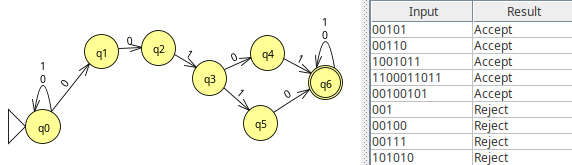
\includegraphics[width=0.9\textwidth]{imgs/189.png}
                \caption{Diagrama de transiciones y validación No. 189.}
        \end{figure}

\end{minipage}
\end{center}

\begin{enumerate}
\setcounter{enumi}{189}
    \item Encuentre un autómata finito no determinista con lenguaje $\Sigma = {0, 1}$ que identifique las palabras que contienen la cadena 11010 y la cadena 10100. Realice el diagrama de transiciones de la palabra 01101010100.
    \begin{center}
        \begin{minipage}{0.45\textwidth}
            \begin{figure}[H]
    		\centering
    		
\includegraphics[width=1.2\textwidth]{imgs/ImgEma/AFN_90.png}
            \end{figure}
            \begin{center}
            \begin{tabular}{c|cc}
            Estado actual & 0 & 1\\
            \hline
            $\rightarrow q0$ & $\{q0\}$ & $\{q0, q1, p1\}$ \\
            $q1$ & $\emptyset$ & $q2$\\
            $q2$ & $q3$ & $\emptyset$\\
            $q3$ & $\emptyset$ & $q4$\\
            $q4$ & $q5$ & $\emptyset$\\
            $q5$ & $\{q5\}$ & $\{q5, q6\}$\\
            $q6$ & $q7$ & $\emptyset$\\
            $q7$ & $\emptyset$ & $q8$\\
            $q8$ & $q9$ & $\emptyset$\\
            $q9$ & $q10$ & $\emptyset$\\
            $*q10$ & $q10$ & $q10$\\
            \hline
            $p1$ & $p2$ & $\emptyset$\\
            $p2$ & $\emptyset$ & $p3$\\
            $p3$ & $p4$ & $\emptyset$\\
            $p4$ & $p5$ & $\emptyset$\\
            $p5$ & $\{p5\}$ & $\{p5, p6\}$\\
            $p6$ & $\emptyset$ & $p7$\\
            $p7$ & $p8$ & $\emptyset$\\
            $p8$ & $\emptyset$ & $p9$\\
            $p9$ & $p10$ & $\emptyset$\\
            $*p10$ & $p10$ & $p10$\\
            \end{tabular}
            \end{center}
        \end{minipage}
        \hfill
        \begin{minipage}{0.45\textwidth}
        Para el ejercicio se requiere que el autómata rastree dos subcadenas diferentes que pueden aparecer en cualquier orden o incluso traslaparse. Para resolverlo como un AFN, usamos el no determinismo para "adivinar" cuándo empieza cada cadena. La estrategia consiste en crear dos rutas: una que busque 11010 y luego 10100, y otra que busque 10100 y luego 11010.\\
        A continuación se define el diagrama de transiciones que sigue el autómata para la palabra: $01101010100$
        \end{minipage}
        \begin{itemize}
            \item \textbf{Inicio}: El autómata comienza en el estado inicial $q_0$.
            \item \textbf{Leer 0}: $\delta(q_0, 0) \to q_0$ (Permanece en el estado inicial).
            \item \textbf{Leer 1}: $\delta(q_0, 1) \to q_1$ (Se activa la rama para buscar la subcadena \texttt{11010}).
            \item \textbf{Leer 1}: $\delta(q_1, 1) \to q_2$ (Segunda '1' detectada).
            \item \textbf{Leer 0}: $\delta(q_2, 0) \to q_3$ ('0' detectado).
            \item \textbf{Leer 1}: $\delta(q_3, 1) \to q_4$ ('1' detectado).
            \item \textbf{Leer 0}: $\delta(q_4, 0) \to q_5$ (\textbf{Subcadena 11010 completada}).
            \item \textbf{Leer 1}: $\delta(q_5, 1) \to q_6$ (Se activa la rama para buscar la subcadena \texttt{10100}).
            \item \textbf{Leer 0}: $\delta(q_6, 0) \to q_7$ ('0' detectado).
            \item \textbf{Leer 1}: $\delta(q_7, 1) \to q_8$ ('1' detectado).
            \item \textbf{Leer 0}: $\delta(q_8, 0) \to q_9$ ('0' detectado).
            \item \textbf{Leer 0}: $\delta(q_9, 0) \to q_{10}$ (\textbf{Subcadena 10100 completada}).
            \item \textbf{Estado Final}: La cadena termina en el estado de aceptación $q_{10}$. \textbf{Cadena Aceptada}.
            \end{itemize}
    \end{center}
\end{enumerate}

\vspace{0.3cm}
\begin{enumerate}
\setcounter{enumi}{190}
\item
En los problemas 191-194, considere el autómata finito no determinista $A = (Q, \Sigma, \delta, A_0, F)$ definido en cada tabla. Encuentre un autómata finito determinista equivalente y realice las siguientes operaciones:
\end{enumerate}

\begin{itemize}
    \item[a)] Calcule $\hat{\delta}(Z,\omega)$, donde $\delta$ es la función de transiciones del autómata.
    \item[b)] Si $\delta_D$ es la función de transición del autómata finito determinista asociado a $A$, calcule $\hat{\delta}_D(Z,\omega)$.
\end{itemize}

Este ejercicio es irresoluble

\vspace{0.5cm}   
\begin{enumerate}
    \setcounter{enumi}{192}
    \item Considere el siguiente autómata no determinista:
\end{enumerate}
    
\begin{center}
    \begin{tabular}{c|cc}
        & 0 & 1 \\
        \hline
        $\rightarrow A$ & $\emptyset$ & $\{B, C\}$ \\
        $B$ & $\{A, D\}$ & $\{B, C, D\}$ \\
        $C$ & $\{C\}$ & $\{A, C\}$ \\
        $*D$ & $\{C\}$ & $\{D\}$ \\
    \end{tabular}
\end{center}
    
    \vspace{0.3cm}
    Realice las operaciones solicitadas:
    
    \begin{itemize}
        \item[a)] $Z = \{A\}, \omega = 01101$
        \item[b)] $Z = \{A, B\}, \omega = 1101$
        \item[c)] $Z = \{C\}, \omega = 1101$
    \end{itemize}

\begin{center}
\begin{minipage}{0.45\textwidth}
\textbf{Solución al Problema 193:}

\vspace{0.3cm}
\textbf{1. Autómata Finito Determinista (AFD) Equivalente} \\
Aplicando el método de construcción de subconjuntos. Se incluyen los estados alcanzables y los subconjuntos requeridos para la evaluación de las cadenas solicitadas.
\begin{center}
    \begin{tabular}{c|cc}
        Estado $\delta_D$ & 0 & 1 \\
        \hline
        $\rightarrow \{A\}$ & $\emptyset$ & $\{B, C\}$ \\
        $\{C\}$ & $\{C\}$ & $\{A, C\}$ \\
        $\{A, B\}$ & $\{A, D\}$ & $\{B, C, D\}$ \\
        $\{A, C\}$ & $\{C\}$ & $\{A, B, C\}$ \\
        $\{B, C\}$ & $\{A, C, D\}$ & $\{A, B, C, D\}$ \\
        $*\{A, D\}$ & $\{C\}$ & $\{B, C, D\}$ \\
        $\{A, B, C\}$ & $\{A, C, D\}$ & $\{A, B, C, D\}$ \\
        $*\{B, C, D\}$ & $\{A, C, D\}$ & $\{A, B, C, D\}$ \\
        $*\{A, C, D\}$ & $\{C\}$ & $\{A, B, C, D\}$ \\
        $*\{A, B, C, D\}$ & $\{A, C, D\}$ & $\{A, B, C, D\}$ \\
        $\emptyset$ & $\emptyset$ & $\emptyset$ \\
    \end{tabular}
\end{center}
\vspace{0.3cm}
\textbf{2. Operaciones solicitadas}

\vspace{0.2cm}
\textbf{a) $Z = \{A\}, \omega = 01101$} \\
\textit{En el AFND ($\hat{\delta}$):} \\
$\hat{\delta}(\{A\}, 0) = \emptyset$ \\
Al llegar al conjunto vacío, cualquier símbolo posterior resulta en $\emptyset$. \\
$\hat{\delta}(\{A\}, 01101) = \emptyset$ \\
\textit{En el AFD ($\hat{\delta}_D$):} \\
$\hat{\delta}_D(\{A\}, 0) = \emptyset \xrightarrow{1101} \emptyset$ \\
\textbf{Resultado:} $\emptyset$



\end{minipage}
\hfill
\begin{minipage}{0.45\textwidth}

\vspace{0.2cm}
\textbf{b) $Z = \{A, B\}, \omega = 1101$} \\
\textit{En el AFND ($\hat{\delta}$):} \\
$\hat{\delta}(\{A, B\}, 1) = \delta(A, 1) \cup \delta(B, 1) = \{B, C\} \cup \{B, C, D\} = \{B, C, D\}$ \\
$\hat{\delta}(\{B, C, D\}, 1) = \delta(B, 1) \cup \delta(C, 1) \cup \delta(D, 1) = \{B, C, D\} \cup \{A, C\} \cup \{D\} = \{A, B, C, D\}$ \\
$\hat{\delta}(\{A, B, C, D\}, 0) = \delta(A, 0) \cup \delta(B, 0) \cup \delta(C, 0) \cup \delta(D, 0) = \emptyset \cup \{A, D\} \cup \{C\} \cup \{C\} = \{A, C, D\}$ \\
$\hat{\delta}(\{A, C, D\}, 1) = \delta(A, 1) \cup \delta(C, 1) \cup \delta(D, 1) = \{B, C\} \cup \{A, C\} \cup \{D\} = \{A, B, C, D\}$ \\
\textit{En el AFD ($\hat{\delta}_D$):} \\
$\hat{\delta}_D(\{A, B\}, 1) = \{B, C, D\}$ \\
$\hat{\delta}_D(\{B, C, D\}, 1) = \{A, B, C, D\}$ \\
$\hat{\delta}_D(\{A, B, C, D\}, 0) = \{A, C, D\}$ \\
$\hat{\delta}_D(\{A, C, D\}, 1) = \{A, B, C, D\}$ \\
\textbf{Resultado:} $\{A, B, C, D\}$

\vspace{0.2cm}
\textbf{c) $Z = \{C\}, \omega = 1101$} \\
\textit{En el AFND ($\hat{\delta}$):} \\
$\hat{\delta}(\{C\}, 1) = \delta(C, 1) = \{A, C\}$ \\
$\hat{\delta}(\{A, C\}, 1) = \delta(A, 1) \cup \delta(C, 1) = \{B, C\} \cup \{A, C\} = \{A, B, C\}$ \\
$\hat{\delta}(\{A, B, C\}, 0) = \delta(A, 0) \cup \delta(B, 0) \cup \delta(C, 0) = \emptyset \cup \{A, D\} \cup \{C\} = \{A, C, D\}$ \\
$\hat{\delta}(\{A, C, D\}, 1) = \delta(A, 1) \cup \delta(C, 1) \cup \delta(D, 1) = \{B, C\} \cup \{A, C\} \cup \{D\} = \{A, B, C, D\}$ \\
\textit{En el AFD ($\hat{\delta}_D$):} \\
$\hat{\delta}_D(\{C\}, 1) = \{A, C\}$ \\
$\hat{\delta}_D(\{A, C\}, 1) = \{A, B, C\}$ \\
$\hat{\delta}_D(\{A, B, C\}, 0) = \{A, C, D\}$ \\
$\hat{\delta}_D(\{A, C, D\}, 1) = \{A, B, C, D\}$ \\
\textbf{Resultado:} $\{A, B, C, D\}$
\end{minipage}

\newpage

\vspace{0.5cm}
\begin{enumerate}
\setcounter{enumi}{194}
\item*
\end{enumerate}

\begin{center}
    \begin{tabular}{c|cc}
         & 0 & 1 \\
        \hline
        $\rightarrow A$ & $\{A, B\}$ & $\{A\}$ \\
        $B$ & $\{A\}$ & $\{C\}$ \\
        $*C$ & $\{A\}$ & $\{D\}$ \\
        $D$ & $\{D\}$ & $\{E\}$ \\
        $*E$ & $\{E\}$ & $\{C, D\}$ \\
    \end{tabular}
\end{center}

\vspace{0.3cm}
Realice las operaciones solicitadas:
\begin{itemize}
    \item[a)] $Z = \{A\}, \omega = 10010$
    \item[b)] $Z = \{A, D\}, \omega = 0110$
    \item[c)] $Z = \{B, E\}, \omega = 0100$
    \item[d)] $Z = \{B, C, D\}, \omega = 10100$
\end{itemize}


\begin{center}
\begin{minipage}{0.45\textwidth}
\textbf{Solución al Problema 195 (Cálculo de $\hat{\delta}(Z,\omega)$):}

\vspace{0.2cm}
\textbf{a) $Z = \{A\}, \omega = 10010$}
\begin{align*}
    \hat{\delta}(\{A\}, 1) &= \{A\} \\
    \hat{\delta}(\{A\}, 0) &= \{A, B\} \\
    \hat{\delta}(\{A, B\}, 0) &= \{A, B\} \cup \{A\} = \{A, B\} \\
    \hat{\delta}(\{A, B\}, 1) &= \{A\} \cup \{C\} = \{A, C\} \\
    \hat{\delta}(\{A, C\}, 0) &= \{A, B\} \cup \{A\} = \{A, B\}
\end{align*}
\textbf{Resultado:} $\{A, B\}$

\vspace{0.2cm}
\textbf{b) $Z = \{A, D\}, \omega = 0110$}
\begin{align*}
    \hat{\delta}(\{A, D\}, 0) &= \{A, B\} \cup \{D\} = \{A, B, D\} \\
    \hat{\delta}(\{A, B, D\}, 1) &= \{A\} \cup \{C\} \cup \{E\} = \{A, C, E\} \\
    \hat{\delta}(\{A, C, E\}, 1) &= \{A\} \cup \{D\} \cup \{C, D\} = \{A, C, D\} \\
    \hat{\delta}(\{A, C, D\}, 0) &= \{A, B\} \cup \{A\} \cup \{D\} = \{A, B, D\}
\end{align*}
\textbf{Resultado:} $\{A, B, D\}$
\end{minipage}
\hfill
\begin{minipage}{0.45\textwidth}

\vspace{0.2cm}
\textbf{c) $Z = \{B, E\}, \omega = 0100$}
\begin{align*}
    \hat{\delta}(\{B, E\}, 0) &= \{A\} \cup \{E\} = \{A, E\} \\
    \hat{\delta}(\{A, E\}, 1) &= \{A\} \cup \{C, D\} = \{A, C, D\} \\
    \hat{\delta}(\{A, C, D\}, 0) &= \{A, B\} \cup \{A\} \cup \{D\} = \{A, B, D\} \\
    \hat{\delta}(\{A, B, D\}, 0) &= \{A, B\} \cup \{A\} \cup \{D\} = \{A, B, D\}
\end{align*}
\textbf{Resultado:} $\{A, B, D\}$

\vspace{0.2cm}
\textbf{d) $Z = \{B, C, D\}, \omega = 10100$}
\begin{align*}
    \hat{\delta}(\{B, C, D\}, 1) &= \{C\} \cup \{D\} \cup \{E\} = \{C, D, E\} \\
    \hat{\delta}(\{C, D, E\}, 0) &= \{A\} \cup \{D\} \cup \{E\} = \{A, D, E\} \\
    \hat{\delta}(\{A, D, E\}, 1) &= \{A\} \cup \{E\} \cup \{C, D\} = \{A, C, D, E\} \\
    \hat{\delta}(\{A, C, D, E\}, 0) &= \{A, B\} \cup \{A\} \cup \{D\} \cup \{E\} = \{A, B, D, E\} \\
    \hat{\delta}(\{A, B, D, E\}, 0) &= \{A, B\} \cup \{A\} \cup \{D\} \cup \{E\} = \{A, B, D, E\}
\end{align*}
\textbf{Resultado:} $\{A, B, D, E\}$
\end{minipage}
\end{center}
\end{center}

\section*{Autómatas finitos no deterministas con transiciones $\lambda$}
Dibuje el diagrama de transiciones de cada uno de los autómatas que se proporcionan en los reactivos 196-200. Encuentre un autómata finito determinista equivalente a cada uno de los que se presentan en los ejercicios, proporcionando su tabla de transiciones y su diagrama de transiciones. Adicionalmente, halle la información que se pide en cada inciso, tomando en cuenta que $\delta$ es la función de transiciones del autómata original.
\newpage
\centering\section*{Expresiones regulares.}
Indique si las afirmaciones 201-238 son verdaderas (V) o falsas (F).

\begin{multicols}{2}
\begin{enumerate}
\setcounter{enumi}{200}

\item $(\ V)\ a \in L(a + b)$
\item $(\ F)\ a \in L(ab)$
\item $(\ V)\ a \in L(a^* + b^*)$
\item $(\ V)\ a \in L(ab^*)$
\item $(\ F)\ aa \in L(a^*b)$
\item $(\ F)\ ab \in L(a + b)$
\item $(\ V)\ ab \in L(ab)$
\item $(\ V)\ ab \in L(a^*b)$
\item $(\ F)\ ab \in L(b^*b)$
\item $(\ V)\ ab \in L((a + b)^*)$
\item $(\ V)\ ab \in L(abc^*)$
\item $(\ F)\ ab \in L(ab^*c)$
\item $(\ V)\ ab \in L(ab^*c^*)$
\item $(\ V)\ ab \in L((a + b + c)^*)$
\item $(\ F)\ ab \in L((abc)^*)$
\item $(\ F)\ ab \in L((ab)^*c)$
\item $(\ F)\ ab \in L(a(bc)^*)$
\item $(\ V)\ ab \in L(a(b + c)^*)$

\columnbreak

\item $(\ F)\ ab \in L((a + b)^*c)$
\item $(\ V)\ ab \in L((a + b)^*c^*)$
\item $(\ F)\ aa \in L(a + b)$
\item $(\ V)\ aa \in L(a^* + b^*)$
\item $(\ V)\ aa \in L(a^*b^*)$
\item $(\ V)\ aa \in L((a + b)^*)$
\item $(\ V)\ aa \in L(a(a + b)^*)$
\item $(\ F)\ \lambda \in L(a)$
\item $(\ V)\ \lambda \in L((a + b)^*)$
\item $(\ V)\ \lambda \in L((a + b)^* + a)$
\item $(\ F)\ \lambda \in L(\emptyset)$
\item $(\ V)\ \lambda \in L(\lambda)$
\item $(\ V)\ \lambda \in L(\lambda + a)$
\item $(\ F)\ \lambda \in L(\lambda a)$
\item $(\ F)\ \lambda \in L(ab^*)$
\item $(\ V)\ \lambda \in L((ab)^*)$
\item $(\ V)\ \emptyset \in L(\emptyset)$

\end{enumerate}
\end{multicols}



\end{document}
